\synctex=1
\documentclass[a4paper,11pt,svgnames]{book}

\usepackage[utf8x]{inputenc}
\usepackage{mathtools}
\usepackage{thesis}
\usepackage{calc}
\usepackage{gensymb}
\usepackage{xspace} 
\setlength{\marginparwidth}{2cm}
\setlength{\voffset}{-0.25in}
\setlength{\parskip}{0.1in}

%\includeonly{5-architecture}
%\includeonly{6-use-case}

%\usepackage{draftwatermark}
%\SetWatermarkScale{4}
\usepackage{subfig}
 \usepackage{listings}
  \usepackage{courier}
 \lstset{
 		 basicstyle=\footnotesize\ttfamily,
         numbers=none,               % Ort der Zeilennummern
         numberstyle=\tiny,          % Stil der Zeilennummern
         %stepnumber=2,               % Abstand zwischen den Zeilennummern
         numbersep=5pt,              % Abstand der Nummern zum Text
         tabsize=2,                  % Groesse von Tabs
         extendedchars=true,         %
         breaklines=true,            % Zeilen werden Umgebrochen
         keywordstyle=\color{red},
    	 frame=single,         
 %        keywordstyle=[1]\textbf,    % Stil der Keywords
 %        keywordstyle=[2]\textbf,    %
 %        keywordstyle=[3]\textbf,    %
 %        keywordstyle=[4]\textbf,   \sqrt{\sqrt{}} %
         stringstyle=\color{white}\ttfamily, % Farbe der String
         showspaces=false,           % Leerzeichen anzeigen ?
         showtabs=false,             % Tabs anzeigen ?
         belowcaptionskip=5pt, 
         xleftmargin=2em, 
         xrightmargin=0.8em,
         %backgroundcolor=\color{lightgray},
         showstringspaces=false      % Leerzeichen in Strings anzeigen ?        
 }
 \lstloadlanguages{% Check Dokumentation for further languages ...
         %[Visual]Basic
         %Pascal
         %C
         %C++
         %XML
         %HP
         Java
 }
    %\DeclareCaptionFont{blue}{\color{blue}} 

  %\captionsetup[lstlisting]{singlelinecheck=false, labelfont={blue}, textfont={blue}}
  \usepackage{caption}
%\DeclareCaptionFont{white}{\color{white}}
%\DeclareCaptionFormat{listing}{\colorbox[HTML]{6DBAFF}{\parbox{\textwidth}{\hspace{5pt}#1#2#3}}}

\DeclareCaptionFont{white}{\color{white}}
\DeclareCaptionFormat{listing}{\colorbox{gray}{\parbox{\textwidth-20pt}{#1#2#3}}\vspace{0.01cm}}
\captionsetup[lstlisting]{format=listing,labelfont=white,textfont=white}

\captionsetup[lstlisting]{format=listing,labelfont=white,textfont=white, singlelinecheck=false, margin=0pt, font={bf,footnotesize}}


\usepackage{url}

%\usepackage[spanish]{babel}
%\usepackage[T1]{fontenc}
\usepackage{tabularx}
\usepackage{graphicx}
\usepackage[usenames,dvipsnames,table]{xcolor}
\usepackage{verbatim}
\usepackage[section]{placeins}
\usepackage{listings}
%\bibliographystyle{unsrt}


\usepackage[pdftex,
    pdfauthor={Unai Arrien Oroz},
            pdftitle={development of a multi-platform mobile musical training software for children using the framework Unity3D engine},
            pdfsubject={Master Thesis},
            pdfkeywords={Unity3D, Application development, Multi-platform development, Game, Mobile},
            pdfproducer={PDFTex},
            colorlinks=true,linkcolor=black,citecolor=black,urlcolor=black,hypertexnames=false]{hyperref}

%\usepackage{longtable}
\setcounter{secnumdepth}{3}

\usepackage{framed}

%lstlisting
\usepackage{listings}

\lstdefinelanguage{JavaScript}{
  keywords={typeof, new, true, false, catch, function, return, null, catch, switch, var, if, in, while, do, else, case, break},
  keywordstyle=\color{blue}\bfseries,
  ndkeywords={class, export, boolean, throw, implements, import, this},
  ndkeywordstyle=\color{darkgray}\bfseries,
  identifierstyle=\color{black},
  sensitive=false,
  comment=[l]{//},
  morecomment=[s]{/*}{*/},
  commentstyle=\color{purple}\ttfamily,
  stringstyle=\color{red}\ttfamily,
  morestring=[b]',
  morestring=[b]"
}

\definecolor{darkblue}{rgb}{0.0,0.0,0.6}

\lstdefinestyle{listXML}{language=XML, basicstyle=\ttfamily\diny, extendedchars=true,  belowcaptionskip=5pt,xleftmargin=0.4em, xrightmargin=0.3em, numbers=none, frame=single, breaklines=true, breakatwhitespace=true, breakindent=0pt, emph={}, emphstyle=\color{red}, basicstyle=\small\ttfamily, columns=fullflexible, showstringspaces=false, commentstyle=\color{gray}\upshape,
morestring=[b]",
morecomment=[s]{<?}{?>},
morecomment=[s][\color{orange}]{<!--}{-->},
keywordstyle=\color{cyan},
stringstyle=\color{black},
tagstyle=\color{darkblue},
morekeywords={xmlns,version,type}
}



\lstdefinestyle{mono}{
   framesep=8px,
   extendedchars=true,
   basicstyle=\ttfamily,
   showstringspaces=false,
   showspaces=false,
   tabsize=2,
   breaklines=true,
   showtabs=false,
   xleftmargin=8pt,
   xrightmargin=8pt
}


\lstdefinestyle{commands}{
   framesep=8px,
   extendedchars=true,
   basicstyle=\ttfamily,
   showstringspaces=false,
   showspaces=false,
   tabsize=2,
   breaklines=true,
   showtabs=false,
   xleftmargin=8pt,
   xrightmargin=8pt
}

\lstdefinestyle{consola}
   {basicstyle=\scriptsize\ttfamily,
    backgroundcolor=\color{white},
    frame=lrtb,
    numbers=none,
    xleftmargin=4pt,
    xrightmargin=4pt
   }


\definecolor{chapterdetails}{HTML}{6DBAFF}

% \usepackage[sf,bf]{titlesec}
% \titleformat{\chapter}[display]
%   {\normalfont\Large\sffamily\raggedleft}
%   {\vspace{5cm}\MakeUppercase{\chaptertitlename}%
%     \rlap{ \resizebox{!}{1.5cm}{\thechapter} \color{chapterdetails}\rule{5cm}{1.5cm}}}
%   {10pt}{\Huge}[{\color{chapterdetails}\titlerule[0.8mm] }]
% \titlespacing*{\chapter}{0pt}{30pt}{20pt}

\usepackage[sf,bf]{titlesec}
\titleformat{\chapter}[display]
  {\normalfont\Large\sffamily\raggedleft}
  {\vspace{5cm}\MakeUppercase{\chaptertitlename}%
    \rlap{ \resizebox{!}{1.5cm}{\thechapter} \color{chapterdetails}\rule{5cm}{1.5cm}}}
  {10pt}{\Huge}[{\color{chapterdetails}\titlerule[0.8mm] }]
\titlespacing*{\chapter}{0pt}{30pt}{20pt}

%\titleformat{\section}{\large\sffamily\bfseries}{\thesection}{1em}{}


\newenvironment{chapterintro}
{% This is the begin code
\large\it
}
{% This is the end code
}


% Tick symbols
\newcommand{\tickYes}{\checkmark}
\newcommand{\tickNo}{\hspace{1pt}\ding{55}}
% Fancy header
\usepackage{fancyhdr}
%Fancy chapter cover style


% Fancy box
\usepackage{fancybox} 
\setlength{\fboxrule}{1 pt} \setlength{\fboxsep}{10pt} \setlength{\shadowsize}{3pt}

%Sky color definition


\begin{document}
\newcommand\litem[1]{\item{\bfseries #1 }}
\renewcommand{\arraystretch}{1.5} %Makes tables less crammed

\newcommand\headcell[1]{%
  \multicolumn{1}{|c|}{\cellcolor{DodgerBlue}\bfseries\sffamily\textcolor{white}{#1}}
}


%Cuadros por tablas
%\renewcommand{\listtablename}{Tables Index}
%\renewcommand{\tablename}{Table} 

% \renewcommand*{\lstlistingname}{List of X}

\pagenumbering{Roman}

\cleardoublepage
\thispagestyle{empty}
\vspace*{3\baselineskip}
{\large{\bf PROYECTO FIN DE CARRERA}}
\vspace{0.5cm}

\begin{rm}
\begin{tabular}{p{3cm}p{10cm}}
\textbf{Título:} & Desarrollo de un Videojuego Móvil Multiplataforma de Educación Infantil Musical utilizando el Entorno de desarrollo Unity3d\\ 
\textbf{Título (inglés):} & Development of a Multi-Platform Mobile Musical Training System for Children using the framework Unity3D Engine\\ 
\textbf{Autor:} & Unai Arríen Oroz \\ 
\textbf{Tutor:} & Carlos A. Iglesias Fernández\\ 
\textbf{Departamento:} & Ingeniería de Sistemas Telemáticos \\ 
\end{tabular} \end{rm} \vspace{1cm}

{\large{\bf MIEMBROS DEL TRIBUNAL CALIFICADOR}} \vspace{0.5cm}

\begin{rm}
\begin{tabular}{p{3cm}p{10cm}}
\textbf{Presidente:} & \\
\textbf{Vocal:} & \\
\textbf{Secretario:} & \\
\textbf{Suplente:} & 
\end{tabular}
\end{rm}
\vspace{1cm}

{\large{\bf FECHA DE LECTURA:}}
\vspace{1cm}

{\large{\bf CALIFICACIÓN:}}
\pagestyle{empty}
\cleardoublepage
\vspace*{\baselineskip}
\begin{center}
	{\LARGE\rm\textbf{UNIVERSIDAD POLITÉCNICA DE MADRID}\\
	\vspace{1.0cm}
	 ESCUELA TÉCNICA SUPERIOR DE\\ INGENIEROS DE TELECOMUNICACIÓN
	  }  \\

	 {\Large\rm Departamento de Ingeniería de Sistemas Telemáticos\\
	 Grupo de Sistemas Inteligentes  }  \\

\begin{figure}[!htbp]
	\centering
    
\includegraphics[width=0.7\textwidth]{img/logo_etsit.jpg}

\end{figure}
	\vspace{1.0cm}
	{{\LARGE\rm PROYECTO FIN DE CARRERA\\
	\vspace{1.0cm}
	 \textbf{DEVELOPMENT OF A MULTI-PLATFORM}\\	 
	 \textbf{MOBILE MUSICAL TRAINING SYSTEM}\\ 
	 \textbf{FOR CHILDREN USING THE FRAMEWORK}\\
	 \vspace{0.5cm}
	 \textbf{UNITY3D ENGINE} }}  \\
	 
	 \vspace{1.0cm}
     \Large\rm\textbf{Unai Arríen Oroz}\\
	 \vspace{1.0cm}
	 Marzo de 2017
\end{center}  

%\cleardoublepage
%
%\begin{tabular}{p{10cm}p{4cm}}
%&\\
%&\\
%&\\
%&\\
%&\\
%&\\
%&\\
%&\\
%&\\
%&\emph{Write cool quote here}\\
%&\\
%\end{tabular}
\cleardoublepage
\phantomsection
\chapter*{Resumen}
\addcontentsline{toc}{chapter}{Resumen}

Esta memoria es el resultado de un proyecto cuyo objetivo es el de desarrollar un videojuego móvil multiplataforma de educación infantil musical utilizando el entorno de desarrollo Unity3D.

Este desarrollo de una aplicación multiplataforma comprende varios procesos: análisis de los requisitos, diseño de la arquitectura, implementación del videojuego, testeo del mismo y despliegue para las plataformas iOs y Android.

Así mismo, se utilizan varios plugins obtenidos a través de la Asset Store de Unity3D, que nos han permitido mejorar el rendimiento del videojuego y facilitar su desarrollo.

Además, se va integra Flurry Analytics como sistema de obtención de métricas y errores de uso de la aplicación para facilitar su posterior mantenimiento.

Por último, se presentan las conclusiones extraídas del trabajo, así como los objetivos que se han alcanzado tras completar el desarollo.

\vfill
\textbf{Palabras clave:} Desarrollo multiplataforma, Desarrollo móvil, Unity3D, Asset Store, Android, iOs, Flurry, 2D Toolkit, HOTtween, Videojuego, Desarrollo software, UML
\cleardoublepage
\phantomsection
\chapter*{Abstract}
\addcontentsline{toc}{chapter}{Abstract}

This thesis is the result of a project whose objective is to develop a multi-platform mobile musical training software for children using the framework Unity3D engine.

This multi-platform development covers several processes: requirement analysis, architecture design, videogame implementation, testing this implementation and iOs and Android deployments.

Moreover, we use plugins obtained through Unity3D Asset Store, which allow us to improve the videogame performance and make its development easier.

Furthermore, we have integrated Flurry Analytics as a metrics an error tool management in order to facilitate future application maintenance.

Finally, we gather the extracted conclusions and check if we achieve the goals defined in the analysis requirement stage.


\vfill
\textbf{Keywords:} Multi-platform development, Mobile development, Unity3D, Asset Store, Android, iOs, Flurry, 2D Toolkit, HOTtween, Videogame, Software development, UML
\cleardoublepage
\phantomsection
\chapter*{Agradecimientos}
\addcontentsline{toc}{chapter}{Agradecimientos}

Quiero aprovechar estas líneas para agradecer a toda la gente que me ha acompañado durante este magnífico \textit{viaje} que tanto he disfrutado.

A mi familia, por su apoyo incondicional y por sus intentos de entender siempre a lo que me dedicaba, a pesar de que raras veces comprendían de que hablaba.

A mis amigos y compañeros de la \textit{Escuela}. A todos aquellos con los que me he cruzado en el camino y me han permitido aprender de ellos. En especial a mis amigos Adrián, Marcos, Juan Fernando, David, Gonzalo y con mención de honor a Beatriz.

Gracias también a mis compañeros de Delegación de Alumnos y de Eurielec, con ellos he aprendido un montón y vivido experiencias inolvidables.

A todos los del Grupo de Sistemas Inteligentes y en especial a Carlos, que siempre ha confiado en mi y me ha apoyado.

A cualquiera que leyendo estas líneas sabe que ha significado algo para mi.
\cleardoublepage
\phantomsection
\addcontentsline{toc}{chapter}{Contents} % para que aparezca en el indice de 
\tableofcontents % indice de contenidos


\cleardoublepage
\phantomsection
\addcontentsline{toc}{chapter}{List of Figures} % para que aparezca en el indice de contenidos
\listoffigures % indice de figuras

\cleardoublepage
\phantomsection
\addcontentsline{toc}{chapter}{List of Tables} % para que aparezca en el indice de contenidos
\listoftables % indice de tablas

\cleardoublepage


%Header style
\pagestyle{fancy}
\fancyhf{}
\fancyhead[RO]{\sffamily \slshape \rightmark}
\fancyhead[LE]{\sffamily \slshape \leftmark}
%\renewcommand{\footrulewidth}{0.4pt} % grosor de la línea del pie
\fancyfoot[OR,EL]{\rmfamily \thepage} % texto derecha del pie
\pagenumbering{arabic}

\cleardoublepage
\chapter{Introduction}

\begin{chapterintro}

This chapters provides an introduction to the problem which will be approached in this project. It provides an overview of the multi-platform application development technologies. Furthermore, a deeper description of the project and its environment is also given.

\end{chapterintro}

\cleardoublepage
\section{Context}

In the last years, mobile devices ecosystem have experimented a huge transformation. These devices have evolved improving their characteristics and changing the way we use them.

Although some of these new features, like an improved performance, have made mobile application development easier, the device market suffers a huge fragmentation which causes lots of problems when we have to deal with multi-platform mobile application developments. This phenomenon, fragmentation, occurs when some mobile users are running different operating systems or different versions of the same operating system (software fragmentation) or when some mobile users are using older devices with less powerful characteristics (hardware fragmentation).

On one hand, the coexistence of different mobile OS such as Android, iOs or Windows Phone and on the other hand the wide range of screen sizes and resolutions make multi-platform mobile application development very complicated. This problem is presented greatly within consulting companies, whose clients requires multi-platform and multi-devices application developments.

When developing native applications, developers implement an application for one specific target platform using its software development kit (SDK) and frameworks. The app is tied to that specific environment. For example, applications for Android are typically programmed in Java, access the platform functionality through Android’s frameworks, and render its user interface by employing platform-provided elements. In contrast, applications for iOS use the program- ming language Objective-C and Apple’s frameworks.

In case multiple platforms are to be supported by native applications, they have to be developed separately for each platform. This approach is the opposite of the cross-platform idea.~\cite{heneval2012}

In order to find a solution, reducing development effort and costs, we need to use multi-platform development tools that allow developers to eliminate the immense effort required to build one mobile applications for each mobile SO we need.

Cross-platform development approaches emerged to address this challenge by allowing developers to implement their apps in one step for a range of platforms, avoiding repetition and increasing productivity.~\cite{heneval2012}

Usually, targeting more than one platform normally requires developing a corresponding application for each mobile operating system. However, this approach means that the development time and hence the cost of the product will increase. A cross-platform approach, on the other hand, helps to solve this problem by developing a single code base that supports multiple platforms. Another benefit of cross-platform development, is that they allow changes to be made faster to portable mobile applications, as only one single code base needs to be modified.~\cite{chaleval2013}

Within the game application development context for multi-platform devices, there are some tools such as Unity3D, Unreal Engine, Marmalade, Autodesk or Corona SDK.

Between all these development tools, Unity3D stands out due its soft learning curve, the possibility of development for multiple platforms in the same project and its huge community.

Moreover, the functions that Unity3D supports autonomously are very abundant. In fact, all game developments are possible such as shader, physics engine, network, terrain manipulation, audio, video, and animation, and it considered so that the revision is possible to the taste of user according to the need.

Unity3D that produces based on Java script and C\# can apply and manage after producing the desired functions with script, not producing all of the programing at once. GUI composed on screen helps the first-time developer to approach easily, and the script and program that programer made with simple mouse drag.~\cite{kim2014dev}

Furthermore, Unity3D Asset Store, which is driven by Unity3D community, includes community plugins which give us an added value.

The proposal of this project is to exemplify the development of a multi-platform mobile musical training software for children using the framework Unity3D Engine.

\section{Master thesis description}

The aim of this master thesis is the development of a multi-platform mobile musical training software for children using the framework Unity3D Engine.

This development has the purpose of training children musical skills. Through physical instrument miniatures which represent the five instrument families (percussion, keyboards, strings, woodwind, brass) the gamer will be able to interact with the application software in three different forms.

Firstly, the gamer will have the possibility to play one instrument of the selected instrument family. Secondly, the gamer will be able to interact with a whole orchestra in order to enable or disable the instruments which will be playing a classical piece. Finally, the gamer will have the possibility to read the history and characteristics of each instrument family.

The multi-platform game development includes all the following development stages:
\begin{itemize}
\item \textit{Requirement analysis}, determining the needs or conditions to meet for the game application.
\item \textit{Architecture design}, defining a structured solution that meets all of the application requirements.
\item \textit{Physical instrument pieces design}, creating the physical pieces that will be used to interact with the application.
\item \textit{Software implementation}, building the multi-platform game using Unity3D engine.
\item \textit{Software test}, testing the application to check if it accomplish the acceptance criteria.
\item \textit{Application deployment}, deploying the application to the needed application markets.
\end{itemize}

Within application architecture we can distinguish the following modules:

\begin{description}

\item[Unity3D engine] is a cross-platform game engine developed by Unity Technologies and used to develop video games for PC, consoles, mobile devices and websites. Unity is notable for its ability to target games to multiple platforms. Within a project, developers have control over delivery to mobile devices, web browsers, desktops, and consoles. Supported platforms include Android, Apple TV, BlackBerry 10, iOS, Linux, Nintendo 3DS line, macOS, PlayStation 4, PlayStation Vita, Unity Web Player (including Facebook), Wii, Wii U, Windows Phone 8, Windows, Xbox 360, and Xbox One.~\cite{unitypress2}

\item[Unity Asset Store] is where a growing library of free and commercial assets are placed. These assets are created both by Unity Technologies and also members of the community. A wide variety of assets is available, covering everything from textures, models and animations to whole project examples, tutorials and Editor extensions. These assets are accessed from a simple interface built into the Unity Editor and are downloaded and imported directly into your project.

\item[Flurry Analytics] enable users to analyze consumer behavior through data observations. The platform provides features for user segmentation, consumer funnels, and applications portfolio analysis. The platform's funnels measure customized consumer conversions and trending metrics, while the portfolio analytics feature allows companies to manage entire portfolios of mobile applications with the ability to monitor data about overlap among applications as well as up-sell and cross-sell conversions.~\cite{flurry1}

\end{description}

\section{Master thesis goals}
\label{sec:masterthesisgoals}

The main purpose of this master thesis is to build a multi-platform mobile musical training software for children using the framework Unity3D Engine.

This multi-platform software includes the software application and the physical miniatures that represent the musical instrument family. The gamer will be able to interact with the software application through these physical instrument pieces.

Regarding the software application, it will have three different game modes which will allow the gamer to play different musical melodies with different musical instruments. Also, the gamer will be able to conduct a whole orchestra and to discover information about all instrument families represented by the physical miniatures instruments.

The multi-platform software development process includes the \textbf{requirement analysis} and the \textbf{architecture design}. Due to the need of physical pieces to interact with the application the build process also include the \textbf{physical instrument pieces design}. After building the game application it has to go through previously designed \textbf{software tests} to check it fits the requirements obtained in the previous stages.

Finally, the application should be deployed to Android and iOs application markets to let users to download and use it, as long as the development team and the client would retrieve metrics and other information about the application use.


\section{Structure of this Master Thesis}

In this section we will provide a brief overview of all the chapters of this Master Thesis. It
has been structured as follows:

\textit{Chapter 1} provides an introduction to the problem which will be approached in this project. It provides an overview of the benefits of Unity3D engine. Furthermore, a deeper description of the project and its environment is also given.

\textit{Chapter 2} contains an overview of the existing technologies on which the development of the project will rely.

\textit{Chapter 3} describes one of the most important stages in software development: the requirement analysis using different scenarios. For this, a detailed analysis of the possible use cases is made using the Unified Modeling Language (UML). This language allows us to specify, build and document a system using graphic language.
The result of this evaluation will be a complete specification of the requirements, which will be matched by each module in the design stage. This helps us also to focus on key aspects and take apart other less important functionalities that could be implemented in future works.

\textit{Chapter 4} describes the architecture of the system, dividing it into two groups and differencing application software development and physical instrument pieces design.

\textit{Chapter 5} describes selected use cases. It is going to be explained the interaction with the whole game going through two of its game modes.

\textit{Chapter 6} sums up the findings and conclusions found throughout the document and gives a hint about the work done for this master thesis.

Finally, the appendix provide useful related information, especially covering the application screens.


\chapter{Enabling Technologies}
\label{chap:enabling_technologies}
\begin{chapterintro}
This chapter introduces which technologies have made possible this project. First of all there must be an engine to build the game application, this is Unity game engine, explained in section \ref{sec:unity}. Secondly, Unity integrates third part software as plugins to facilitate development through its Asset Store, this components are detailed in section \ref{sec:assetstore}. Finally, there should be a tool to manage application metrics and information after its deployment, this is done by Flurry Analytics, explained in section \ref{sec:flurry}.
\end{chapterintro}

\cleardoublepage
\section{Unity3D game engine}
\label{sec:unity}
Today’s game creators rely on game engines to develop the main pieces of software for their games. A game engine simplifies the task of the programmers by offering convenient abstractions for the hardware and operating systems on top of which the game runs.~\cite{messaoudi2015dis}

Gamers play on so many different types of devices which have lots of differences regarding their hardware and software resources. One of the main purposes of a game engine is to make this development easier avoiding building one application for each device we want to be compatible with.

Unity3D game engine is an integrated development tool for producing other interactive contents such as video game, architectural visualization, real-time 3D animation. Its editor runs on Window, Mac OS X, so it could make games as the platforms of Window, Mac, Wii, iPad, and iPhone. It could also produce web browser game that uses unity web player plug-in. This is a similar form of flash, and it is designed so that flash user could easily adapt even with cross domain security policy and scripting.

The functions that Unity3D supports autonomously are very abundant. In fact, all game developments are possible such as shader, physics engine, network, terrain manipulation, audio, video, and animation, and it considered so that the revision is possible to the taste of user according to the need. Unity3D that produces based on Java script and C\# can apply and manage after producing the desired functions with script, not producing all of the programing at once. GUI composed on screen helps the first-time developer to approach easily, and the script and program that programer made with simple mouse drag.~\cite{kim2014dev}

\begin{figure}[h]
\centering

\includegraphics[width=200pt]{graphics/enabling-tech/unity_logo.png}
\caption{Unity3D logo}
\label{fig:unity_logo}
\end{figure}

Unity3D is a flexible and high-performance development platform used to make creative and intelligent interactive 3D and 2D experiences. The "author once, deploy everywhere" capability ensures developers can publish to all of the most popular platforms. Unity Technologies boasts a thriving community of over 2 million developers including large publishers, indie studios, students and hobbyists. To remain at the forefront of innovation, Unity Technologies tirelessly re-invests in its award-winning 3D development tools and its democratization initiatives, such as the Asset Store digital content marketplace and Unity Games publishing and distribution division.~\cite{unitypress1}

We will detail Unity3D components and how those components will be integrated in the application development in the following subsections. Frstly we will detail Unity3D principal features in \ref{subsec:unityfeatures}, secondly in \ref{subsec:unityinterface} we are going to explain Unity3D interface from where we create our game and finally in \ref{subsec:unitycomponents} we are going to explain all the components seen on that interface:

\subsection{Unity3D features}
\label{subsec:unityfeatures}
The latest update, Unity 4.6, was released in August, 2012. It currently supports development for iOS, Android, Windows, OS X, Linux, web browsers, Flash, PlayStation 3, Xbox 360, and Wii U.~\cite{unitypress2} The game engine can be downloaded from their website in two different versions: Unity and Unity Pro. Between its features we can point highlight the following:
\begin{itemize}
\item \textit{Rendering}, The graphics engine uses Direct3D (Windows), OpenGL (Mac, Windows,
Linux), OpenGL ES (Android, iOS), and proprietary APIs (Wii). There is support for bump mapping, reflection mapping, parallax mapping, screen space ambient occlusion (SSAO), dynamic shadows using shadow maps, render-to-texture and full-screen post-processing effects.
Unity supports art assets and file formats from 3ds Max, Maya, Softimage, Blender, Modo, ZBrush, Cinema 4D, Cheetah3D, Adobe Photoshop, Adobe Fireworks and Allegorithmic Substance. These assets can be added to the game project, and managed through Unity's graphical user interface.~\cite{unitypress3}
The ShaderLab language is used for shaders, supporting both declarative "programming" of the fixed-function pipeline and shader programs written in GLSL or Cg. A shader can include multiple variants and a declarative fallback specification, allowing Unity to detect the best variant for the current video card, and if none are compatible, fall back to an alternative shader that may sacrifice features for performance.~\cite{unitypress4}
\item \textit{Scripting}, The game engine's scripting is built on Mono, the open-source implementation
of the .NET Framework. Programmers can use UnityScript (a custom language with ECMAScript-inspired syntax), C\# or Boo (which has a Python-inspired syntax).~\cite{unitypress5} Starting with the 3.0 release, Unity ships with a customized version of MonoDevelop for debugging scripts.~\cite{unitypress6}
\item \textit{Asset Tracking}, Unity also includes the Unity Asset Server, a version control solution for the developer's game assets and scripts. It uses PostgreSQL as a backend, an audio system built on the FMOD library (with ability to playback Ogg Vorbis compressed audio), video playback using the Theora codec, a terrain and vegetation engine (which supports tree billboarding, Occlusion Culling with Umbra), built-in lightmapping and global illumination with Beast, multiplayer networking using RakNet, and built-in pathfinding navigation meshes.~\cite{unitypress7}
\item \textit{Platforms}, Unity supports deployment to multiple platforms. Within a project, developers
have control over delivery to mobile devices, web browsers, desktops, and consoles.~\cite{unitypress2}
Unity also allows specification of texture compression and resolution settings for each platform the game supports.~\cite{unitypress2}
Currently supported platforms include Windows, Linux, Mac, Android, iOS, Unity Web Player, Adobe Flash, PlayStation 3, Xbox 360, and Wii. Although not officially confirmed, Unity also supports the PlayStation Vita as can be seen on the game Escape Plan. Upcoming platforms include BlackBerry 10, Wii U, Windows 8, and Windows Phone 8.
\item \textit{Asset Store}, Launched in November 2010, the Unity Asset Store is a resource available
within the Unity editor. The store consists of a collection of over 4,400 asset packages, including 3D models, textures and materials, particle systems, music and sound effects, tutorials and projects, scripting packages, editor extensions and online services. We will detail this feature in section \ref{sec:assetstore}. The store also contains many extensions, tools and asset packages such as the package 2D Toolkit, which provides an efficient \& flexible 2D sprite, collider set-up, text, tilemap and UI system integrating seamlessly into the Unity environment.
\item \textit{Versions}, The first version of Unity was launched at Apple’s Worldwide Developers Conference in 2005. It was built to function and build projects on Mac computers and garnered enough success to continue development of the engine and tools for other platforms.[2] Unity 3 was released in September 2010 and focused on introducing more of the tools that high-end studios have at their disposal. This allowed the company to capture the interest of bigger developers while providing independent and smaller teams with a game engine in one affordable package. The latest version of Unity, Unity 4.6, was released in August 2014, and includes features such as New UI System: Design UIs for your game or application using Unity's powerful new component based UI framework and visual tools and an extensible event messaging system.
\end{itemize}

\subsection{Unity3D interface}
\label{subsec:unityinterface}
When we create a project, the first thing we see is Unity3D interface. This interface can be easily customized so that it would fits developer needs. In figure \ref{fig:unity_interface_general} we can see the interface that we have to used during the game development process.

\begin{figure}[h]
\centering
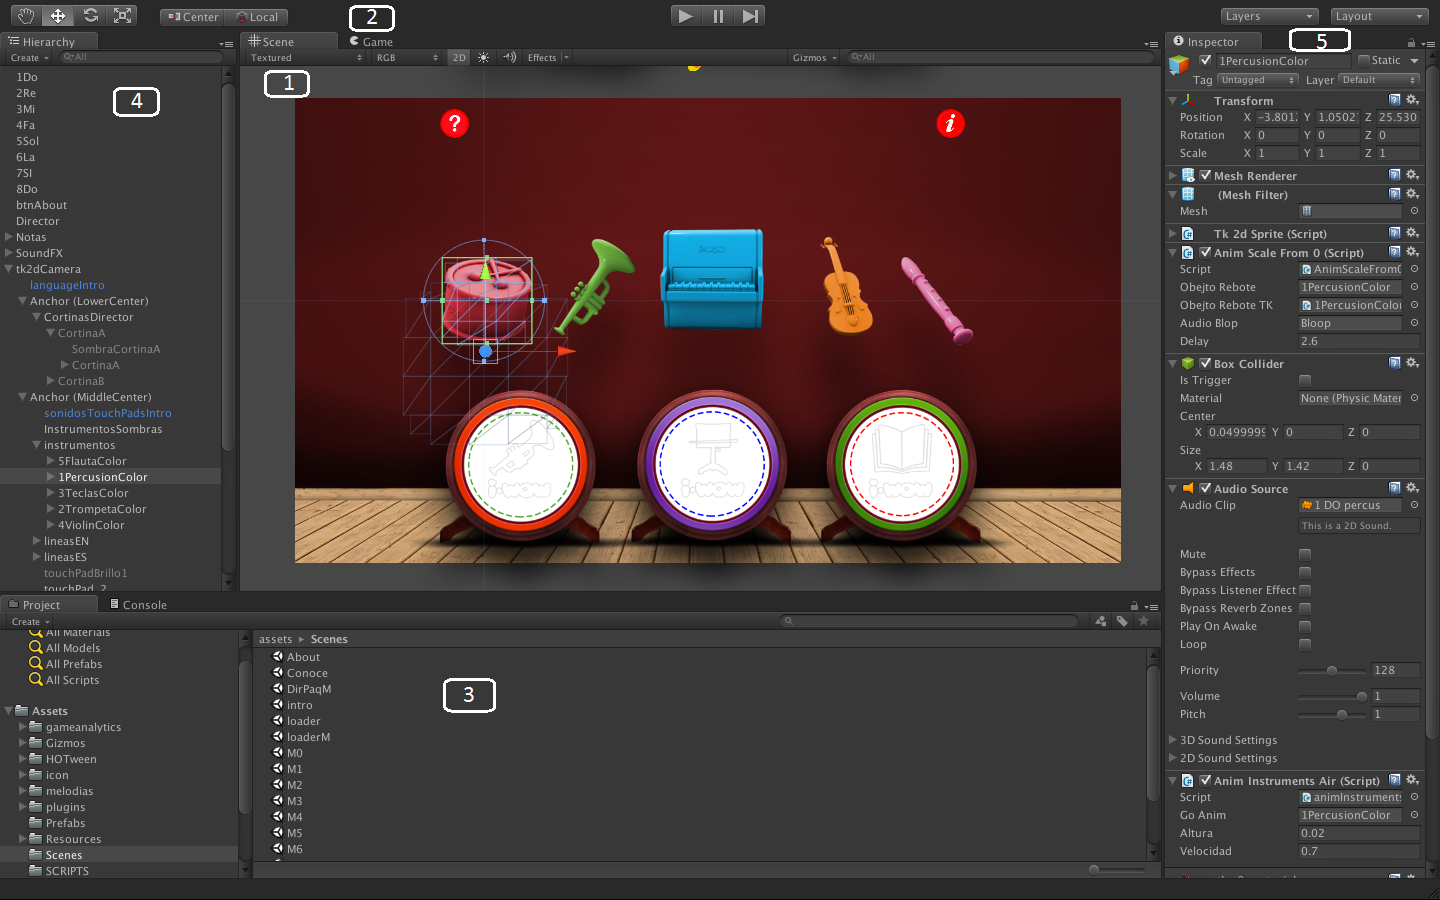
\includegraphics[width=450pt]{graphics/enabling-tech/unity_interface_general.png}
\caption{Unity3D interface}
\label{fig:unity_interface_general}
\end{figure}

\subsection{Unity3D components}
\label{subsec:unitycomponents}

\section{Unity Asset Store}
\label{sec:assetstore}


\section{Flurry analytics}
\label{sec:flurry}

\chapter{Requirement Analysis}
\label{chap:requirements}

\begin{chapterintro}
This chapter describes one of the most important stages in software development: the requirement analysis using different scenarios. For this, a detailed analysis of the possible use cases is made using the Unified Modeling Language (UML). This language allows us to specify, build and document a system using graphic language. 
\end{chapterintro}


\cleardoublepage

\section{Overview}
The result of this chapter will be a complete specification of the requirements, which will be matched by each module in the design stage. This helps us also to focus on key aspects and take apart other less important functionalities that could be implemented in future works.

%As commented before, our project aims to develop a personal assistance system that integrates the advantages of agent systems, information retrieval and Natural Language Processing. Our personal assistant should have the capability to solve user's questions using all of these features.

\section{Use cases}

These sections identify the use cases of the system. This helps us to obtain a complete specification of the uses of the system, and therefore define the complete list of requisites to match.  First, we will present a list of the actors in the system and a UML diagram representing all the actors participating in the different use cases. This representation allows, apart from specifying the actors that interact in the system, the relationships between them.

These use cases will be described the next sections, including each one a table with their complete specification. Using these tables, we will be able to define the requirements to be established.


\subsection{Actors dictionary}

\noindent The list of primary and secondary actors is presented in table \ref{tab:actores}. These actors participate in the different use cases, which are presented later.\\



\begin{table}[!htpb]
\centering
\begin{tabular}{|c|c|x{6cm}|}
\noalign{\hrule height 2pt}
\textbf{Actor identifier} & \textbf{Role} & \textbf{Description}\tn
\hline
ACT-1 & Gamer & End user that play the game using the physical instruments and the application\tn
\hline
ACT-2 & Instrument recognition algorithm & Algorithm that detects what physical figure has been placed on the application recognition zones\tn
\hline
ACT-3 & Client & Company that have outsourced the game development\tn
\hline
ACT-4 & Flurry & Tecnhology that manage application metrics and errors\tn
\noalign{\hrule height 2pt}
\end{tabular}
\caption{Actors list}
\label{tab:actores}
\end{table}


\clearpage


\FloatBarrier


\subsection{Game modes use case}
This use case package collects the game play modes and their functionalities, as shown in \ref{fig:pack-uc1}.

The use cases presented in this section are as shown in the Figure \ref{fig:pack-uc1}:
\begin{itemize}
\item \textit{play instrument} detailed in sub-section \ref{subsec:playinstrument}.
\item \textit{conducte orchestra} detailed in sub-section \ref{subsec:conducteorchestra}.
\item \textit{discover instrument}  detailed in sub-section \ref{subsec:discoverinstrument}.
\item \textit{watch demo}  detailed in sub-section \ref{subsec:watchdemo}.
\item \textit{select melody}  detailed in sub-section \ref{subsec:selectmelody}.
\item \textit{select instrument}  detailed in sub-section \ref{subsec:selectinstrument}.
\end{itemize}


\begin{figure}[h]
\centering
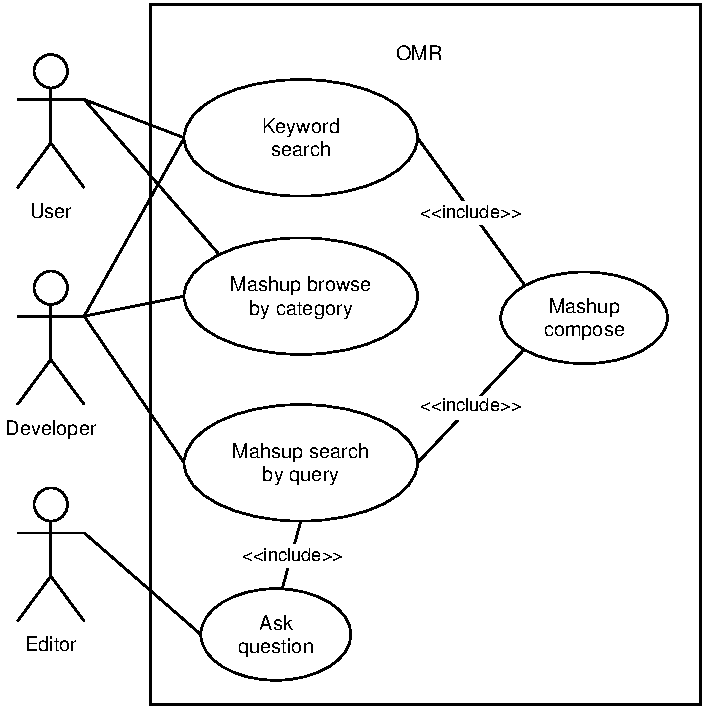
\includegraphics[width=400pt]{graphics/uc1.pdf}
\caption{Game modes use case}
\label{fig:pack-uc1}
\end{figure}

\newpage
\subsubsection{Play instrument}
\label{subsec:playinstrument}

\begin{table}[!htpb]
\centering
\begin{tabular}{|c|x{1cm}x{5cm}x{5cm}|}
\noalign{\hrule height 2pt}
\textbf{Use Case Name} & \multicolumn{3}{c|}{play instrument}\\
\hline
\textbf{Use Case ID} & \multicolumn{3}{x{11cm}|}{UC1.1}\\
\hline
\textbf{Primary Actor} & \multicolumn{3}{c|}{Gamer}\\
\hline
\textbf{Pre-Condition} & \multicolumn{3}{x{11cm}|}{The application is showing the home screen and the gamer has the instruments physical miniatures}\\
\hline
\textbf{Post-Condition} & \multicolumn{3}{x{11cm}|}{Optionally, the gamer can watch a demo, change the instrument or change the melody}\\
\hline
\textbf{Flow of Events} & \multicolumn{1}{c|}{} & \multicolumn{1}{x{5cm}|}{Actor Input} & \multicolumn{1}{x{5cm}|}{System Response}\\
\hline

\textbf{} & \multicolumn{1}{x{0.5cm}|}{1} & \multicolumn{1}{x{5cm}|}{The gamer put an instrument miniature on home screen. The instrument is placed in the detection zone circle that represents the play instrument game mode} & \multicolumn{1}{x{5cm}|}{The application load the play instrument mode game with the instrument that have been placed on the screen and the default melody. }\\
\hline

\end{tabular}
\end{table}

\FloatBarrier

\newpage
\subsubsection{Conducte orchestra}
\label{subsec:conducteorchestra}


\begin{table}[!htpb]
\centering
\begin{tabular}{|c|x{1cm}x{5cm}x{5cm}|}
\noalign{\hrule height 2pt}
\textbf{Use Case Name} & \multicolumn{3}{c|}{conducte orchestra}\\
\hline
\textbf{Use Case ID} & \multicolumn{3}{x{11cm}|}{UC1.2}\\
\hline
\textbf{Primary Actor} & \multicolumn{3}{c|}{Gamer}\\
\hline
\textbf{Pre-Condition} & \multicolumn{3}{x{11cm}|}{The application is showing the home screen and the gamer has the instruments physical miniatures}\\
\hline
\textbf{Post-Condition} & \multicolumn{3}{x{11cm}|}{Optionally, the gamer can play, stop or change the melody, enable or disable an instrument and change the instrument family}\\
\hline
\textbf{Flow of Events} & \multicolumn{1}{c|}{} & \multicolumn{1}{x{5cm}|}{Actor Input} & \multicolumn{1}{x{5cm}|}{System Response}\\
\hline

\textbf{} & \multicolumn{1}{x{0.5cm}|}{1} & 
\multicolumn{1}{x{5cm}|}{The gamer put an instrument miniature on home screen. The instrument is placed in the detection zone circle that represents the conduct orchestra game mode} & 
\multicolumn{1}{x{5cm}|}{The application load the conduct orchestra game mode with all instruments enabled, the family instrument selector of the family instrument that have been placed on the screen enabled, and the default melody.}\\
\hline

\end{tabular}
\end{table}
\FloatBarrier

\newpage
\subsubsection{Discover instrument}
\label{subsec:discoverinstrument}

\FloatBarrier

\begin{table}[!htpb]
\centering
\begin{tabular}{|c|x{1cm}x{5cm}x{5cm}|}
\noalign{\hrule height 2pt}
\textbf{Use Case Name} & \multicolumn{3}{c|}{discover instrument}\\
\hline
\textbf{Use Case ID} & \multicolumn{3}{x{11cm}|}{UC1.3}\\
\hline
\textbf{Primary Actor} & \multicolumn{3}{c|}{Gamer}\\
\hline
\textbf{Pre-Condition} & \multicolumn{3}{x{11cm}|}{The application is showing the home screen and the gamer has the instruments physical miniatures}\\
\hline
\textbf{Post-Condition} & \multicolumn{3}{x{11cm}|}{Optionally, the gamer can play the an instrument sound and change the instrument family}\\
\hline
\textbf{Flow of Events} & \multicolumn{1}{c|}{} & \multicolumn{1}{x{5cm}|}{Actor Input} & \multicolumn{1}{x{5cm}|}{System Response}\\
\hline

\textbf{} & \multicolumn{1}{x{0.5cm}|}{1} & 
\multicolumn{1}{x{5cm}|}{The gamer put an instrument miniature on home screen. The instrument is placed in the detection zone circle that represents the discover instrument game mode} & 
\multicolumn{1}{x{5cm}|}{The application load the discover instrument game mode with the instruments of the family instrument that have been placed on the screen. The game mode shows instrument information and sounds}\\
\hline

\end{tabular}
\end{table}

\FloatBarrier

\newpage
\subsubsection{Watch demo}
\label{subsec:watchdemo}


\begin{table}[!htpb]
\centering
\begin{tabular}{|c|x{1cm}x{5cm}x{5cm}|}
\noalign{\hrule height 2pt}
\textbf{Use Case Name} & \multicolumn{3}{c|}{watch demo}\\
\hline
\textbf{Use Case ID} & \multicolumn{3}{x{11cm}|}{UC1.4}\\
\hline
\textbf{Primary Actor} & \multicolumn{3}{c|}{Gamer}\\
\hline
\textbf{Pre-Condition} & \multicolumn{3}{x{11cm}|}{Play instrument game mode has been selected}\\
\hline
\textbf{Post-Condition} & \multicolumn{3}{x{11cm}|}{-}\\
\hline
\textbf{Flow of Events} & \multicolumn{1}{c|}{} & \multicolumn{1}{x{5cm}|}{Actor Input} & \multicolumn{1}{x{5cm}|}{System Response}\\
\hline

\textbf{} & \multicolumn{1}{x{0.5cm}|}{1} & 
\multicolumn{1}{x{5cm}|}{The gamer touch Demo button with a selected melody and instrument} & 
\multicolumn{1}{x{5cm}|}{The melody in played with the instrument selected and musical notes are highlated}\\
\hline


\end{tabular}
\end{table}
\FloatBarrier

\newpage
\subsubsection{Select melody}
\label{subsec:selectmelody}

\begin{table}[!htpb]
\centering
\begin{tabular}{|c|x{1cm}x{5cm}x{5cm}|}
\noalign{\hrule height 2pt}
\textbf{Use Case Name} & \multicolumn{3}{c|}{select melody}\\
\hline
\textbf{Use Case ID} & \multicolumn{3}{x{11cm}|}{UC1.5}\\
\hline
\textbf{Primary Actor} & \multicolumn{3}{c|}{Gamer}\\
\hline
\textbf{Pre-Condition} & \multicolumn{3}{x{11cm}|}{Play instrument game mode or conduct orchestra have been selected}\\
\hline
\textbf{Post-Condition} & \multicolumn{3}{x{11cm}|}{-}\\
\hline
\textbf{Flow of Events} & \multicolumn{1}{c|}{} & \multicolumn{1}{x{5cm}|}{Actor Input} & \multicolumn{1}{x{5cm}|}{System Response}\\
\hline

\textbf{} & \multicolumn{1}{x{0.5cm}|}{1} & 
\multicolumn{1}{x{5cm}|}{The gamer touch Melodies button} & 
\multicolumn{1}{x{5cm}|}{A list of the melodies are shown}\\
\hline

\textbf{} & \multicolumn{1}{x{0.5cm}|}{2} & 
\multicolumn{1}{x{5cm}|}{The gamer chose one of the avaiable melodies} & 
\multicolumn{1}{x{5cm}|}{Selected melody is loaded into game mode}\\
\hline

\end{tabular}
\end{table}
\FloatBarrier

\newpage
\subsubsection{Select instrument}
\label{subsec:selectinstrument}

\begin{table}[!htpb]
\centering
\begin{tabular}{|c|x{1cm}x{5cm}x{5cm}|}
\noalign{\hrule height 2pt}
\textbf{Use Case Name} & \multicolumn{3}{c|}{select instrument}\\
\hline
\textbf{Use Case ID} & \multicolumn{3}{x{11cm}|}{UC1.6}\\
\hline
\textbf{Primary Actor} & \multicolumn{3}{c|}{Gamer}\\
\hline
\textbf{Secondary Actor} & \multicolumn{3}{c|}{Instrument recognition algorithm}\\
\hline
\textbf{Pre-Condition} & \multicolumn{3}{x{11cm}|}{Any game mode is selected and the gamer has the instruments physical miniatures}\\
\hline
\textbf{Post-Condition} & \multicolumn{3}{x{11cm}|}{O-}\\
\hline
\textbf{Flow of Events} & \multicolumn{1}{c|}{} & \multicolumn{1}{x{5cm}|}{Actor Input} & \multicolumn{1}{x{5cm}|}{System Response}\\
\hline

\textbf{} & \multicolumn{1}{x{0.5cm}|}{1} & 
\multicolumn{1}{x{5cm}|}{The Gamer place the instrument in the circle recognition zone} & 
\multicolumn{1}{x{5cm}|}{The Instrument recognition algorithm process the instrument pad touches and determine which instrument have been placed}\\
\hline

\textbf{} & \multicolumn{1}{x{0.5cm}|}{2} & 
\multicolumn{1}{x{5cm}|}{The Instrument recognition algorithm detect a different instrument} & 
\multicolumn{1}{x{5cm}|}{Selected instrument is loaded into game mode}\\
\hline

\end{tabular}
\end{table}
\FloatBarrier

\newpage
\subsection{Game managment use case}
This use case package collects the main managment use cases of the game, as shown in \ref{fig:pack-uc2}

\begin{itemize}
\item \textit{metrics managment} detailed in subsection \ref{subsec:metricsmanagment}
\item \textit{errors managment} detailed in subsection \ref{subsec:errorsmanagment}
\end{itemize}

\begin{figure}[h]
\centering
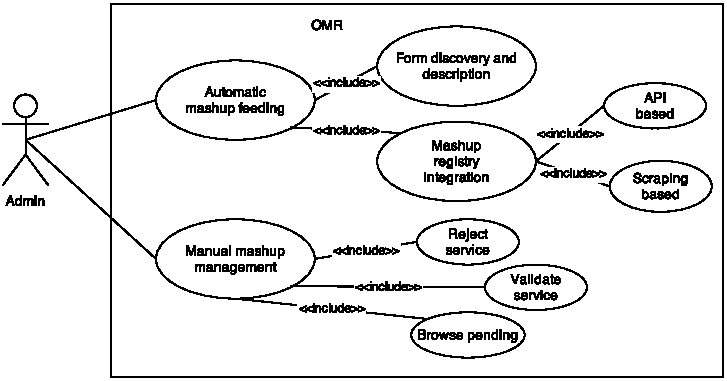
\includegraphics[width=400pt]{graphics/uc2.pdf}
\caption{Game managment use case}
\label{fig:pack-uc2}
\end{figure}

\FloatBarrier

\newpage
\subsubsection{Metrics managment}
\label{subsec:metricsmanagment}

\begin{table}[!htpb]
\centering
\begin{tabular}{|c|x{1cm}x{5cm}x{5cm}|}
\noalign{\hrule height 2pt}
\textbf{Use Case Name} & \multicolumn{3}{c|}{Metrics managment}\\
\hline
\textbf{Use Case ID} & \multicolumn{3}{x{11cm}|}{UC2.1}\\
\hline
\textbf{Primary Actor} & \multicolumn{3}{c|}{Client}\\
\hline
\textbf{Secondary Actor} & \multicolumn{3}{c|}{Flurry}\\
\hline
\textbf{Pre-Condition} & \multicolumn{3}{x{11cm}|}{Flurry client account has been created. Application is running}\\
\hline
\textbf{Post-Condition} & \multicolumn{3}{x{11cm}|}{Metrics are added to Flurry servers}\\
\hline
\textbf{Flow of Events} & \multicolumn{1}{c|}{} & \multicolumn{1}{x{5cm}|}{Actor Input} & \multicolumn{1}{x{5cm}|}{System Response}\\
\hline

\textbf{} & \multicolumn{1}{x{0.5cm}|}{1} & 
\multicolumn{1}{x{5cm}|}{The client access to their Flurry acount} & 
\multicolumn{1}{x{5cm}|}{Flurry shows all metrics included with their SDK in the application}\\
\hline

\end{tabular}
\end{table}
\FloatBarrier

\newpage
\subsubsection{Errors managment}
\label{subsec:errorsmanagment}

\begin{table}[!htpb]
\centering
\begin{tabular}{|c|x{1cm}x{5cm}x{5cm}|}
\noalign{\hrule height 2pt}
\textbf{Use Case Name} & \multicolumn{3}{c|}{Metrics managment}\\
\hline
\textbf{Use Case ID} & \multicolumn{3}{x{11cm}|}{UC2.2}\\
\hline
\textbf{Primary Actor} & \multicolumn{3}{c|}{Client/Developer}\\
\hline
\textbf{Secondary Actor} & \multicolumn{3}{c|}{Flurry}\\
\hline
\textbf{Pre-Condition} & \multicolumn{3}{x{11cm}|}{Flurry client and developer accounts has been created. Application is running and an error has been thrown}\\
\hline
\textbf{Post-Condition} & \multicolumn{3}{x{11cm}|}{Errors are sent to Flurry servers}\\
\hline
\textbf{Flow of Events} & \multicolumn{1}{c|}{} & \multicolumn{1}{x{5cm}|}{Actor Input} & \multicolumn{1}{x{5cm}|}{System Response}\\
\hline

\textbf{} & \multicolumn{1}{x{0.5cm}|}{1} & 
\multicolumn{1}{x{5cm}|}{The client and the developers access to their Flurry acount} & 
\multicolumn{1}{x{5cm}|}{Flurry shows all errors included with their SDK in the application}\\
\hline

\end{tabular}
\end{table}
\FloatBarrier

\subsection{Conclusions}

With the use cases described we have introduced the basic functionalities that have been implemented in this project. They help us to understand the different actors that can interact. They can serve as a base for further development and different use cases that can come to mind.
\chapter{Architecture}
\label{chap:architecture}


\begin{chapterintro}
This chapter describes in depth how the system is structured in different modules and how the users interact with them and also how the modules interact with other modules by themselves.
\end{chapterintro}

\cleardoublepage
\section{Architecture Overview}
In this section we will describe the \textbf{videogame architecture}, starting with its two main modules, the \textbf{physical instruments miniatures} and the \textbf{software application}. In Figure \ref{fig:ArchitectureGeneral} we show the global game architecture identifying both main modules and their relation.

\begin{figure}[ht!]
	\centering
	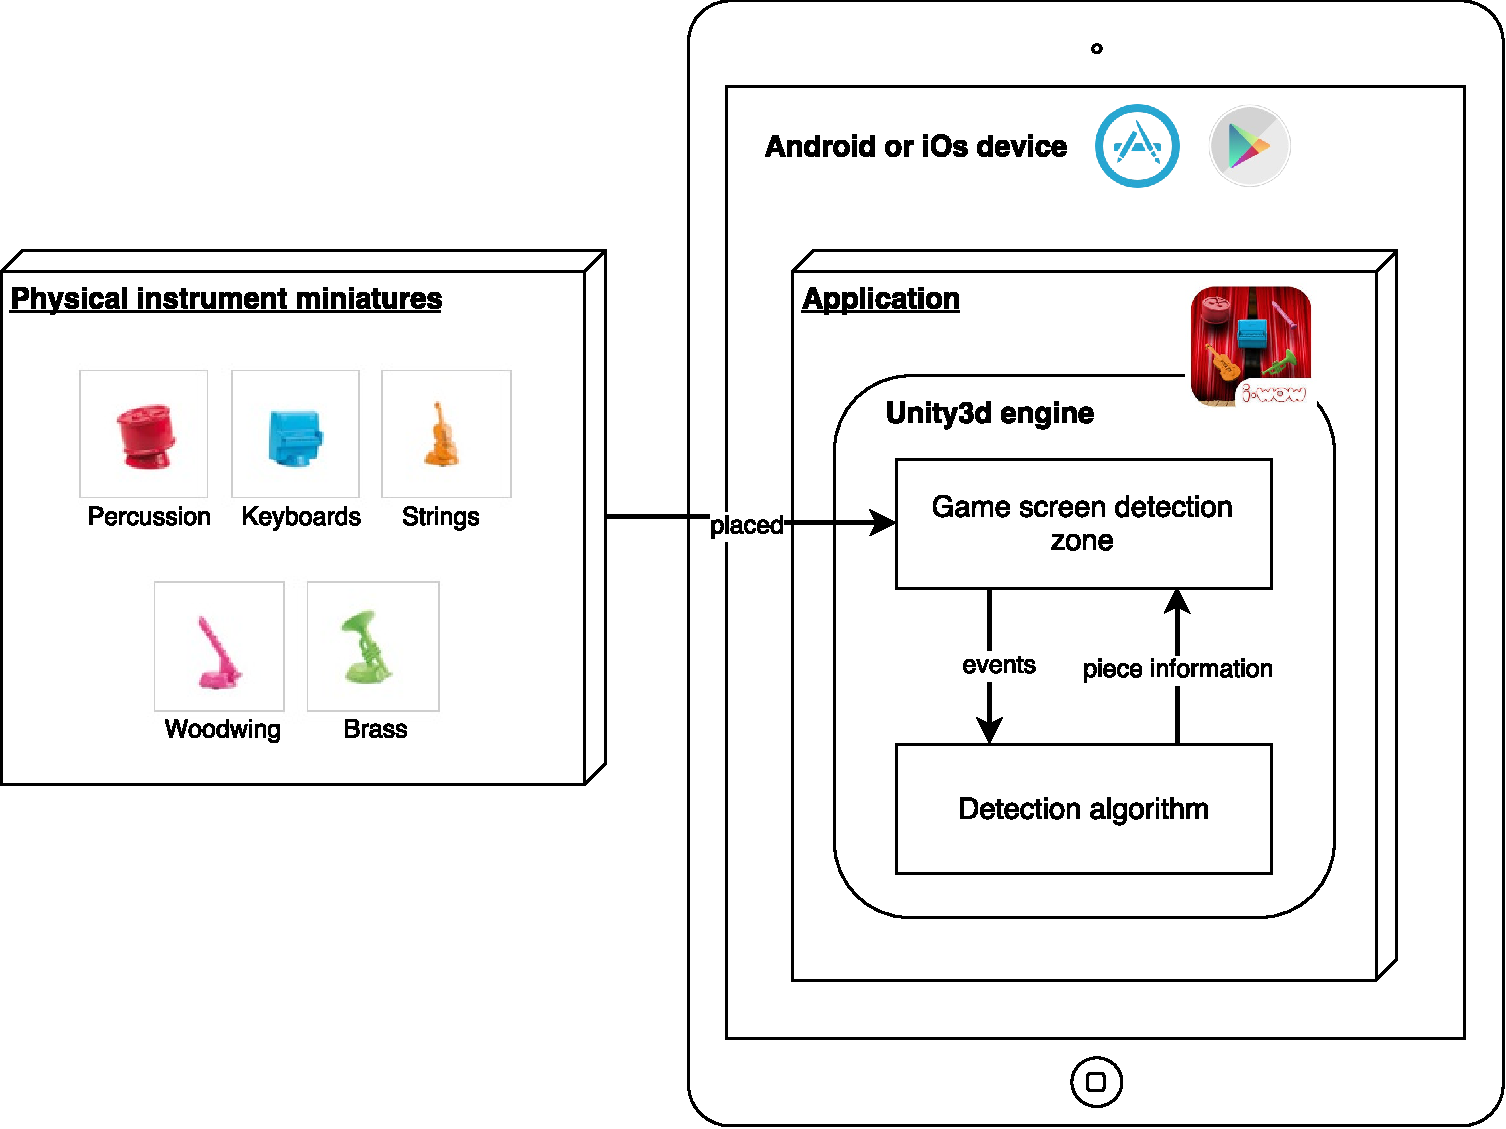
\includegraphics[width=400pt]{graphics/architecture/ArchitectureGeneral.pdf}
	\caption{General Architecture}
	\label{fig:ArchitectureGeneral}
\end{figure}

\FloatBarrier

The modules are detailed below:

\subsection{Physical instruments miniatures}
There are five physical miniatures which represent each one of the musical instrument families used at the game: percussion, keyboards, strings, woodwind and brass. The gamer will use these pieces to interact with the app in order to change or activate the family represented by the piece. Also, pieces will be used to access to different game modes.

The interaction between the pieces and the app is haptic, that is, the gamer will pick a miniature and they will place it in the “instrument detection zone” represented by a shiny circle in the app screen. The app “detection algorithm” will determine which piece has been placed and will make an event depending on the game mode and the app state. These events are, for example, changing instrument, activate instrument, etc.

Each piece base has three little pads which conform a triangle used to determine the instrument unequivocally.

Instrument miniatures design will be explain in more detail in section \ref{sec:instrumentminuatures}

\subsection{Application}
The application has been developed using Unity, so we can identify the Unity components included on our app. These components are Unity Scenes, Unity Textures, Unity Assets, Unity Scripts and Unity Sounds. Integrating all of these components into our Unity projects we are able to build the game logic and its graphic interface.

Unity is notable for its ability to target games to multiple platforms. Within a project, we have control over delivery to different mobile devices, web browsers, desktops, and consoles. In our case, we need to develop both Android and iOs applications and Unity allow us to share the same code for them. Also, using Unity Android and iOs Plugins we are able to access to native Android and iOs SDKs, in case we need to access to some Android or iOs native components.

The application architecture will be explain in more detail in section \ref{sec:application}

\FloatBarrier

\section{Physical instruments miniatures}
\label{sec:instrumentminuatures}
Besides the application software development, our videogame included five \textit{physical instruments miniatures}. These pieces are used by the gamer to interact with the application.

The interaction is simple, the gamer place one of the pysical pieces on one of the several recognition zones displayed within the game screens. Placing these pieces, the gamer is able to select or enable an instrument belonging to the family represented by the physical miniature.

As we said before, we have five pieces:
\begin{itemize}
\item \textit{Drum}, which represents the \textit{percussion} instrument family, shown in Figure \ref{fig:percussionpiece}.
\item \textit{Piano}, which represents the \textit{keyboards} instrument family, shown in Figure \ref{fig:keyboardspiece}.
\item \textit{Violin}, which represents the \textit{strings} instrument family, shown in Figure \ref{fig:stringspiece}.
\item \textit{Flute}, which represents the \textit{woodwind} instrument family, shown in Figure \ref{fig:woodwindpiece}.
\item \textit{Trumpet}, which represents the \textit{brass} instrument family, shown in Figure \ref{fig:brasspiece}.
\end{itemize}

\begin{figure}[ht!]
	\centering
	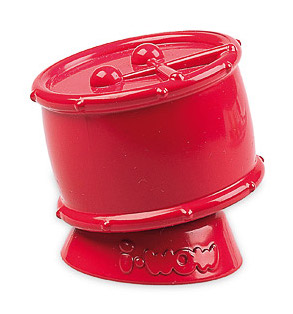
\includegraphics[width=100pt]{graphics/architecture/pieces/piecePercussion.jpg}
	\vspace{0.6cm}
	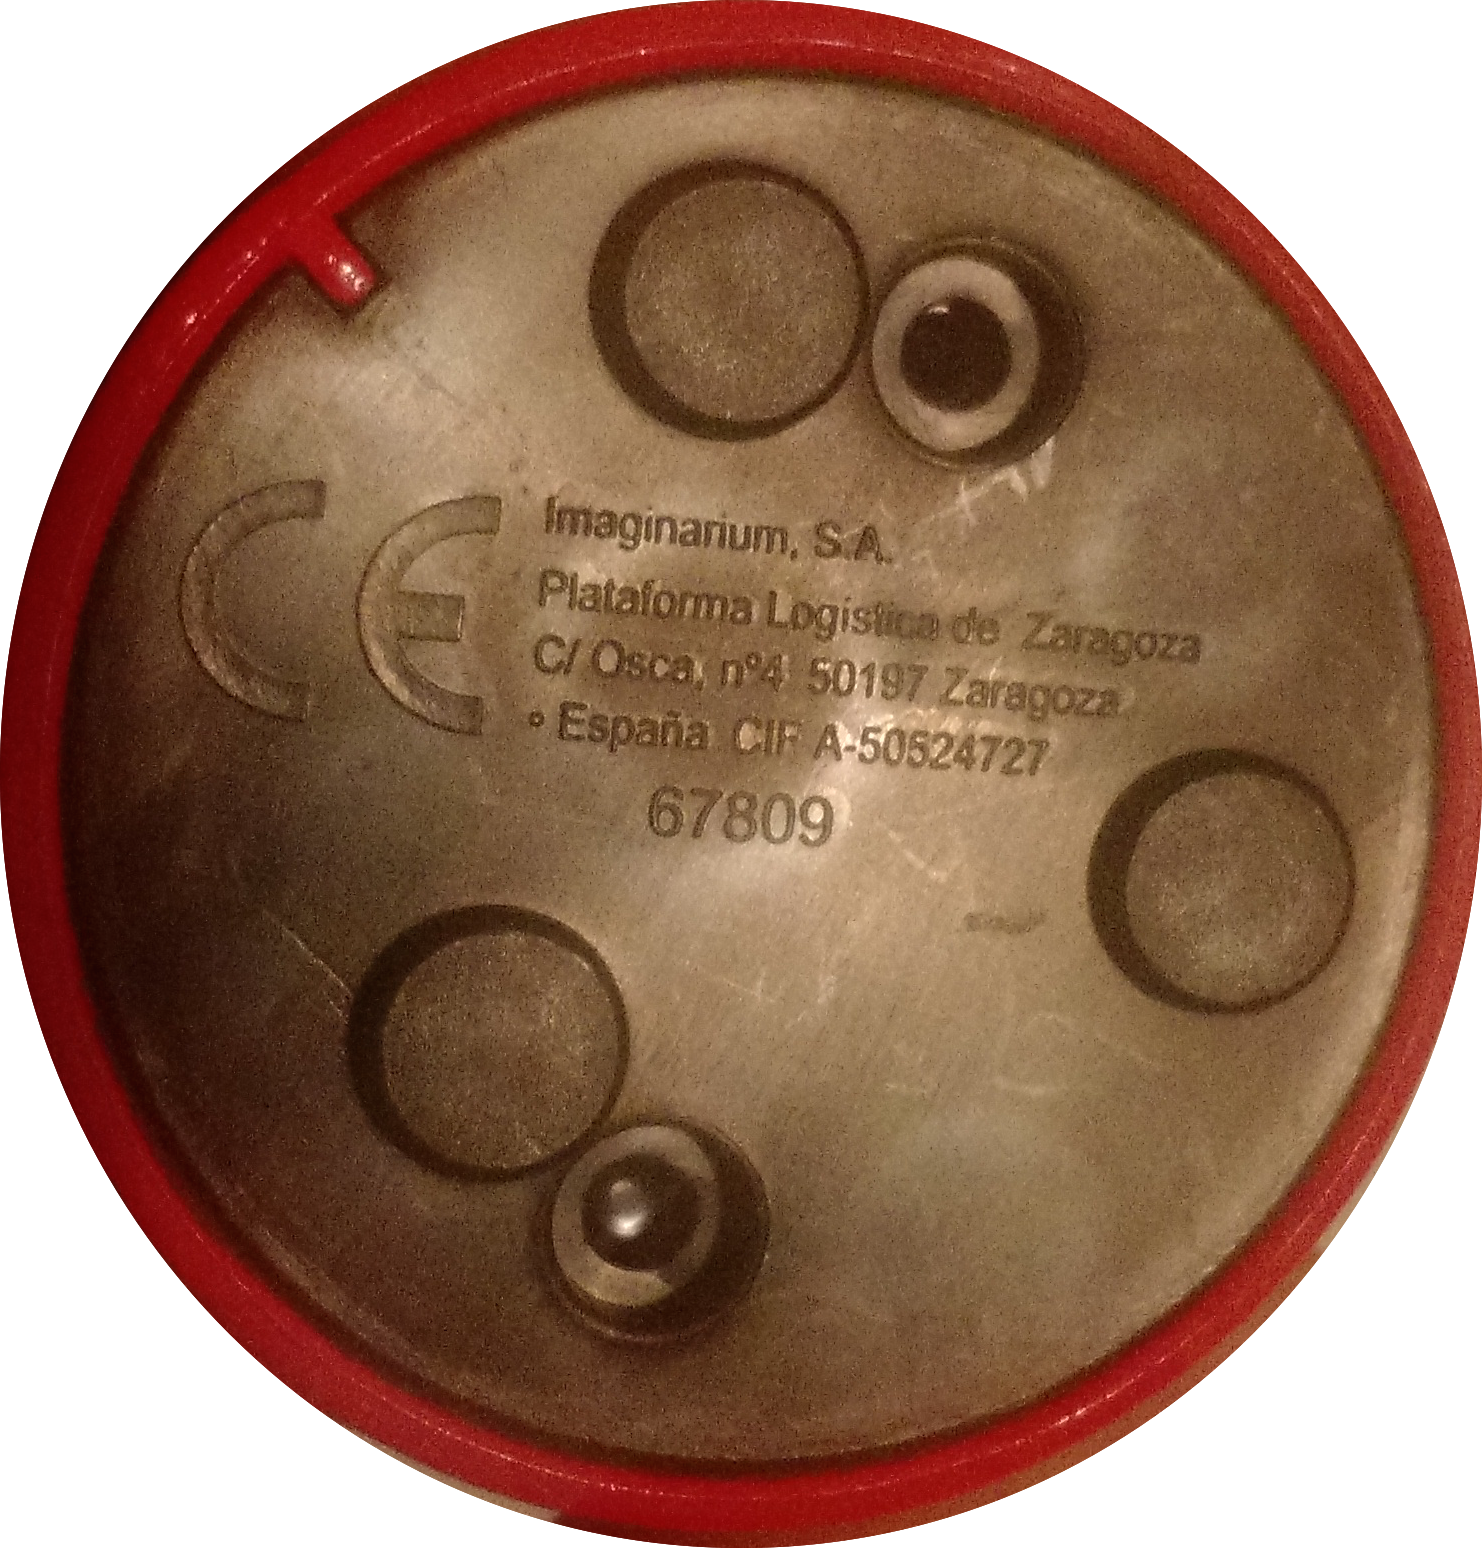
\includegraphics[width=100pt]{graphics/architecture/pieces/percussionBase.png}
	\caption{Drum piece (frontal and base). It represents the percussion family}
	\label{fig:percussionpiece}
\end{figure}

\begin{figure}[ht!]
	\centering
	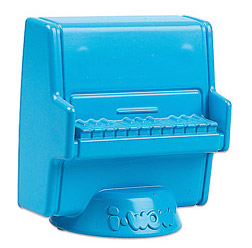
\includegraphics[width=100pt]{graphics/architecture/pieces/pieceKeyboards.jpg}
	\vspace{0.6cm}
	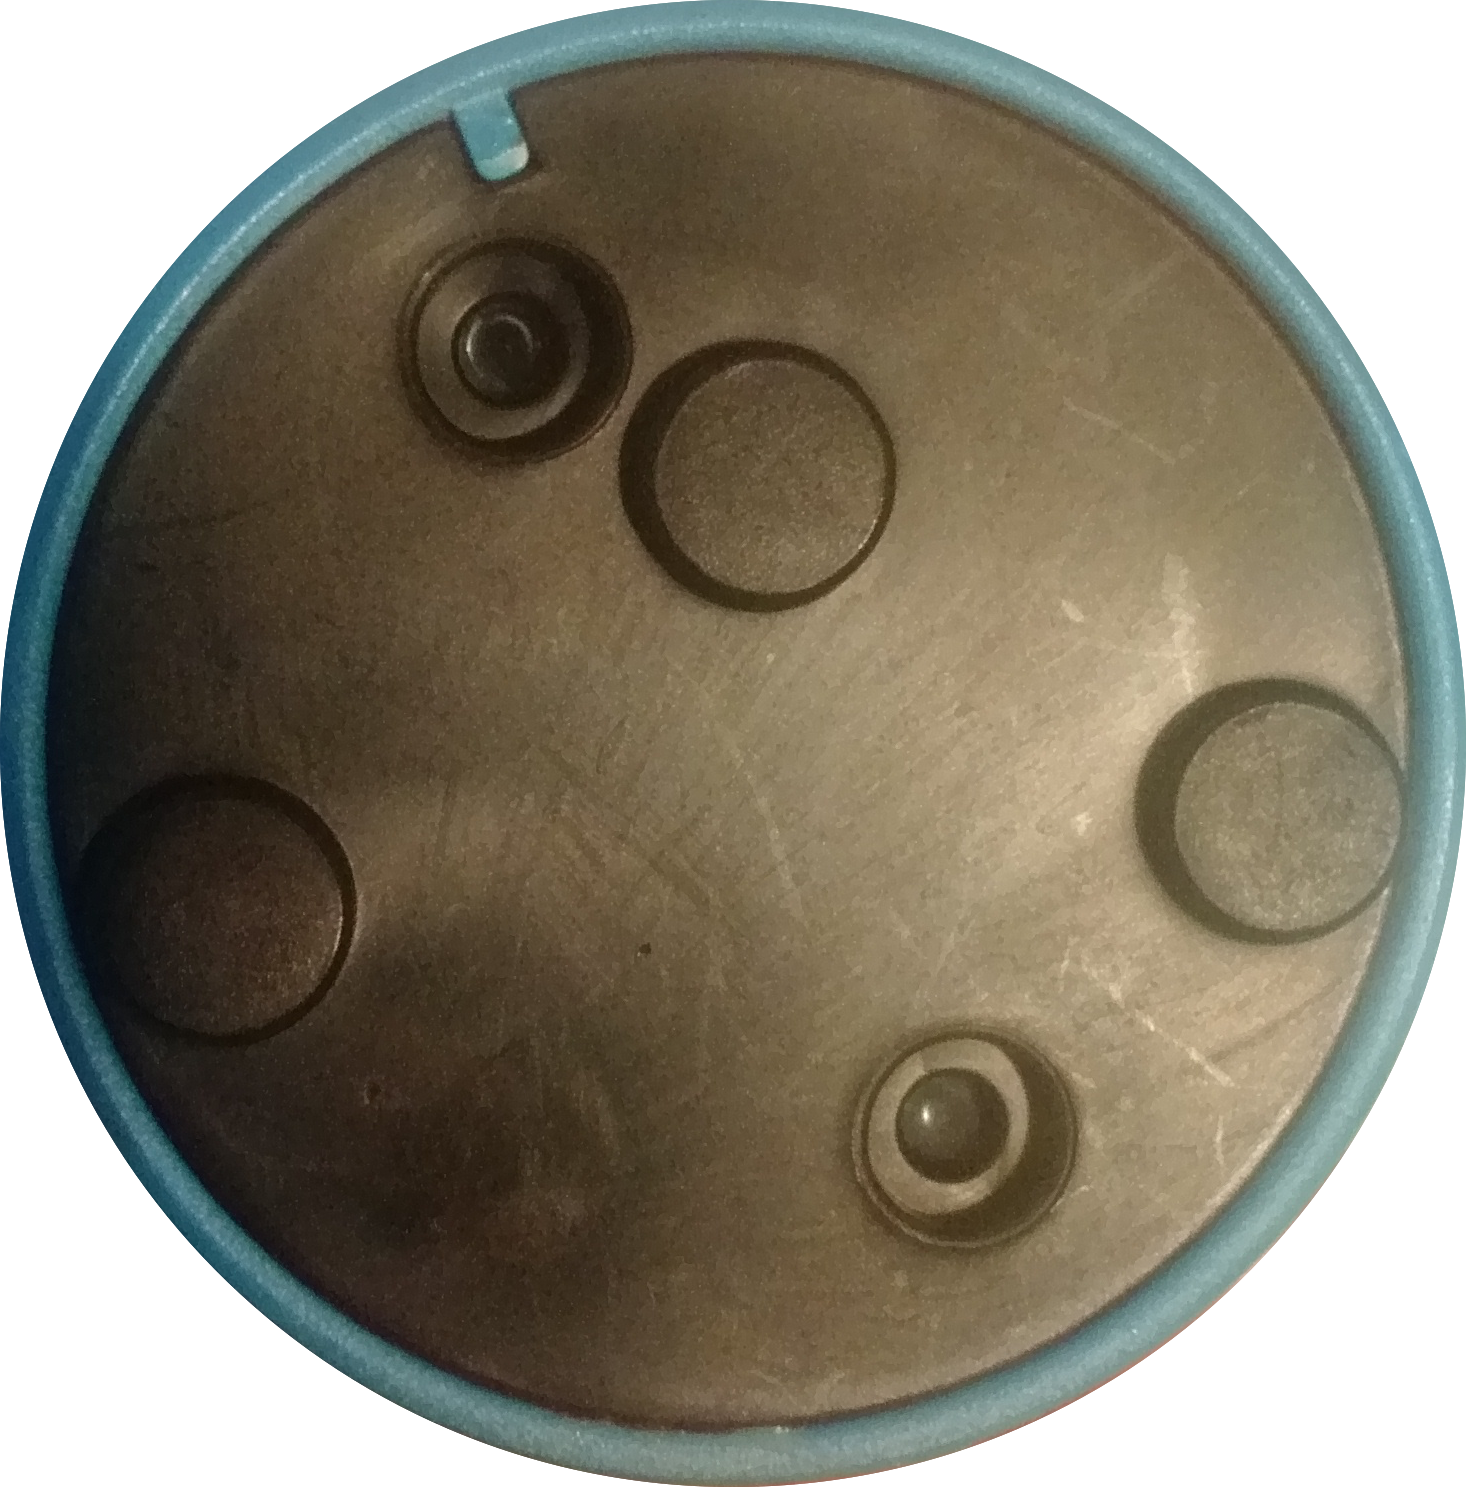
\includegraphics[width=100pt]{graphics/architecture/pieces/keyboardsBase.png}
	\caption{Piano piece (frontal and base). It represents the keyboards family}
	\label{fig:keyboardspiece}
\end{figure}

\begin{figure}[ht!]
	\centering
	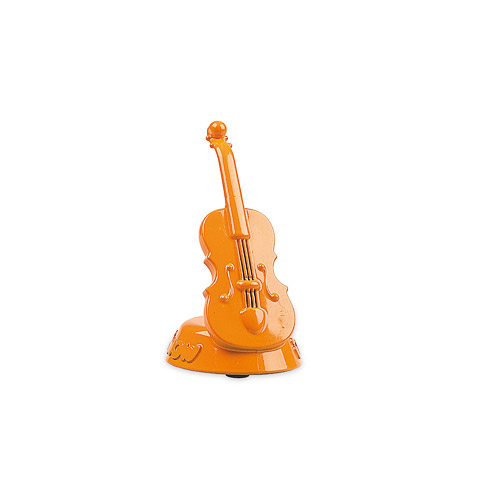
\includegraphics[width=100pt]{graphics/architecture/pieces/pieceStrings.jpg}
	\vspace{0.6cm}
	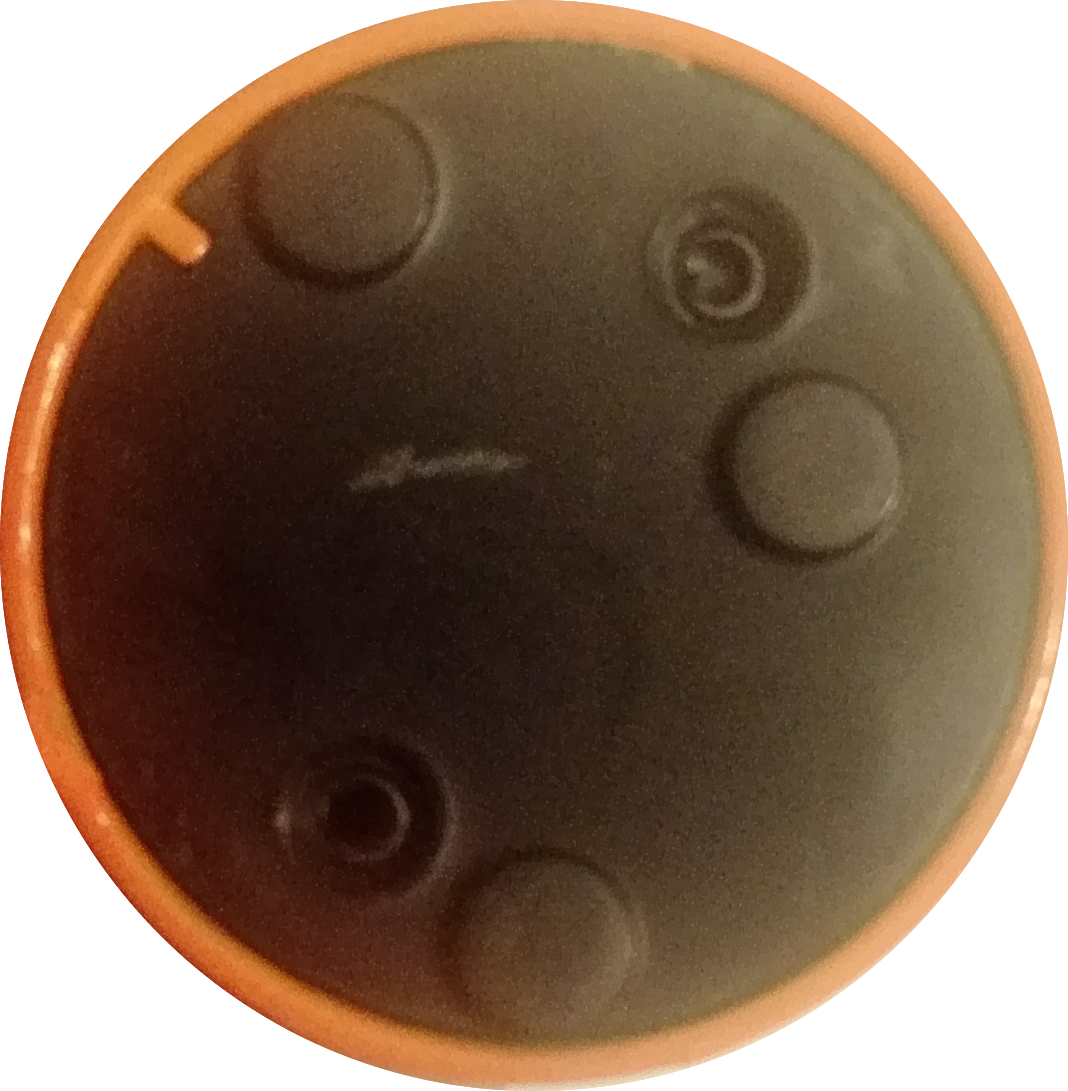
\includegraphics[width=100pt]{graphics/architecture/pieces/stringsBase.png}
	\caption{Violin piece (frontal and base). It represents the string family}
	\label{fig:stringspiece}
\end{figure}

\begin{figure}[ht!]
	\centering
	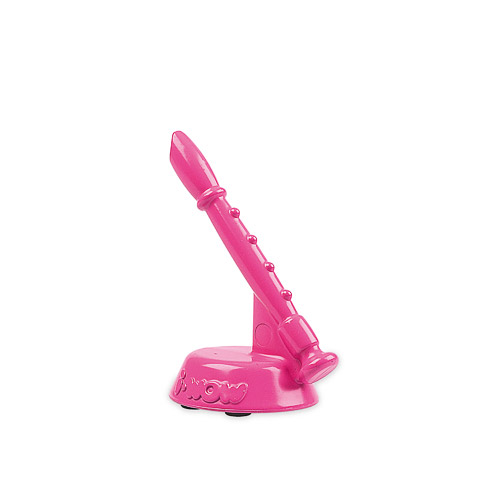
\includegraphics[width=100pt]{graphics/architecture/pieces/pieceWoodwind.jpg}
	\vspace{0.6cm}
	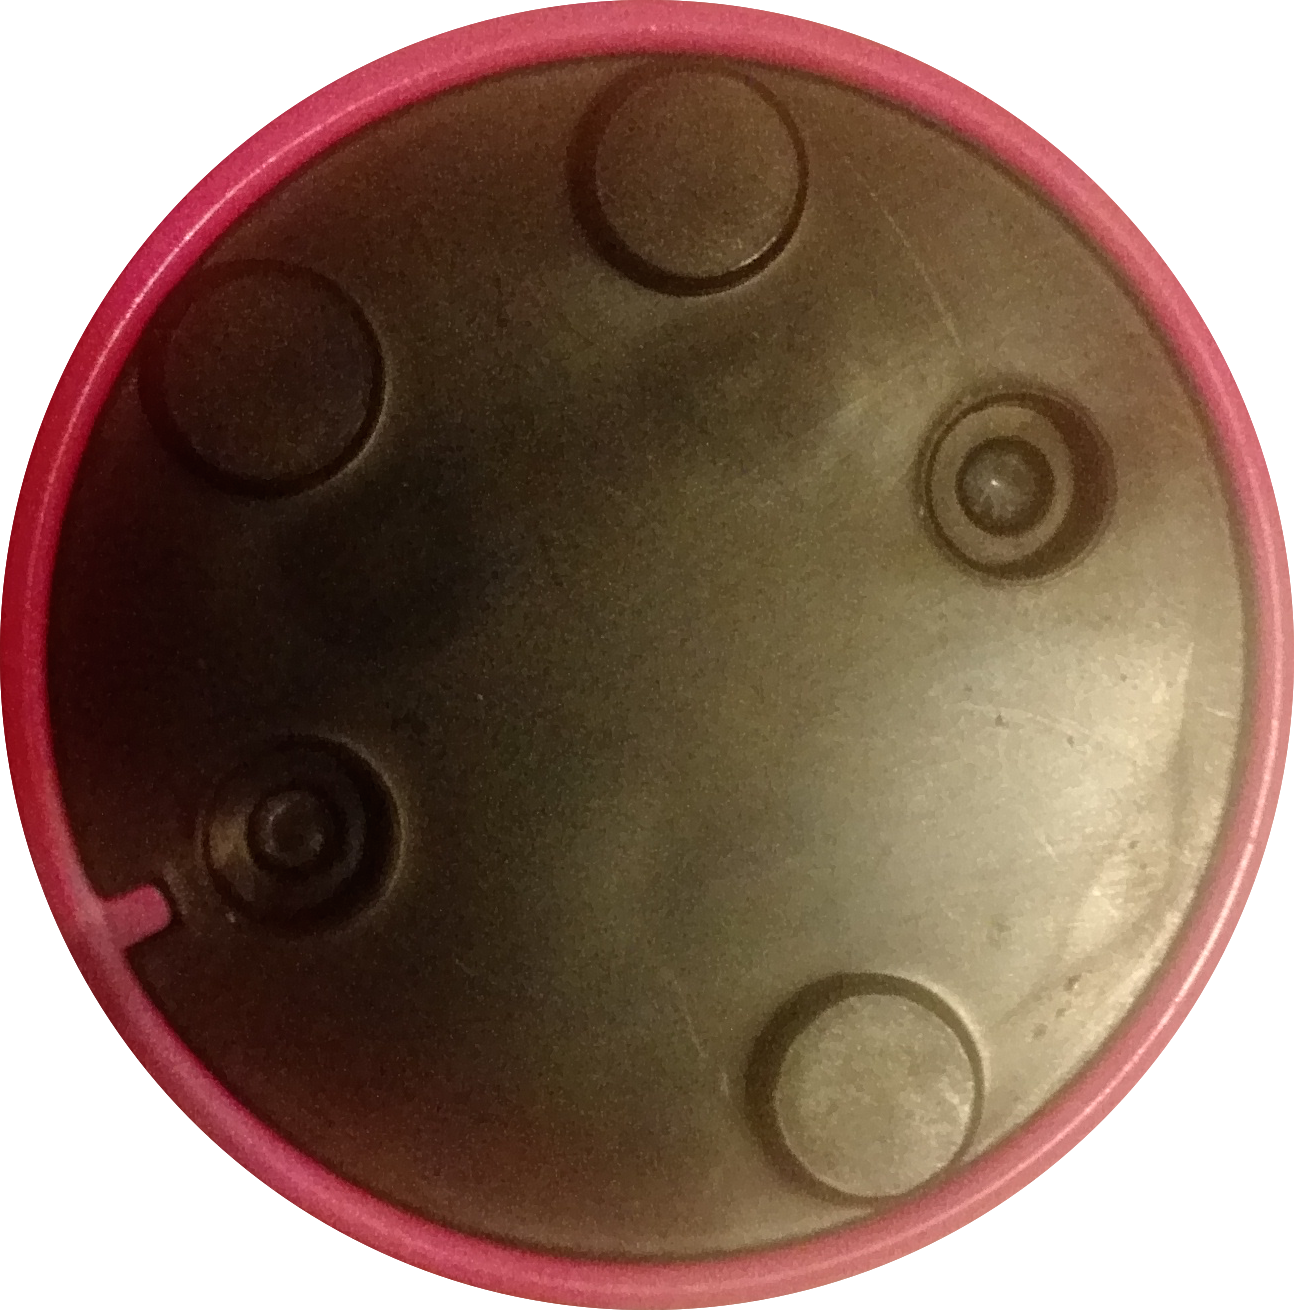
\includegraphics[width=100pt]{graphics/architecture/pieces/woodwindBase.png}
	\caption{Flute piece (frontal and base). It represents the woodwind family}
	\label{fig:woodwindpiece}
\end{figure}

\begin{figure}[ht!]
	\centering
	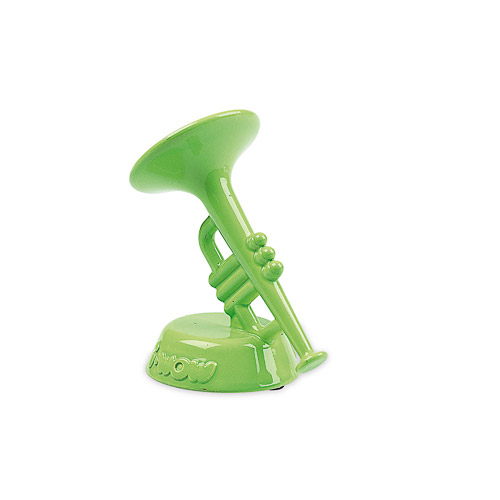
\includegraphics[width=100pt]{graphics/architecture/pieces/pieceBrass.jpg}
	\vspace{0.6cm}
	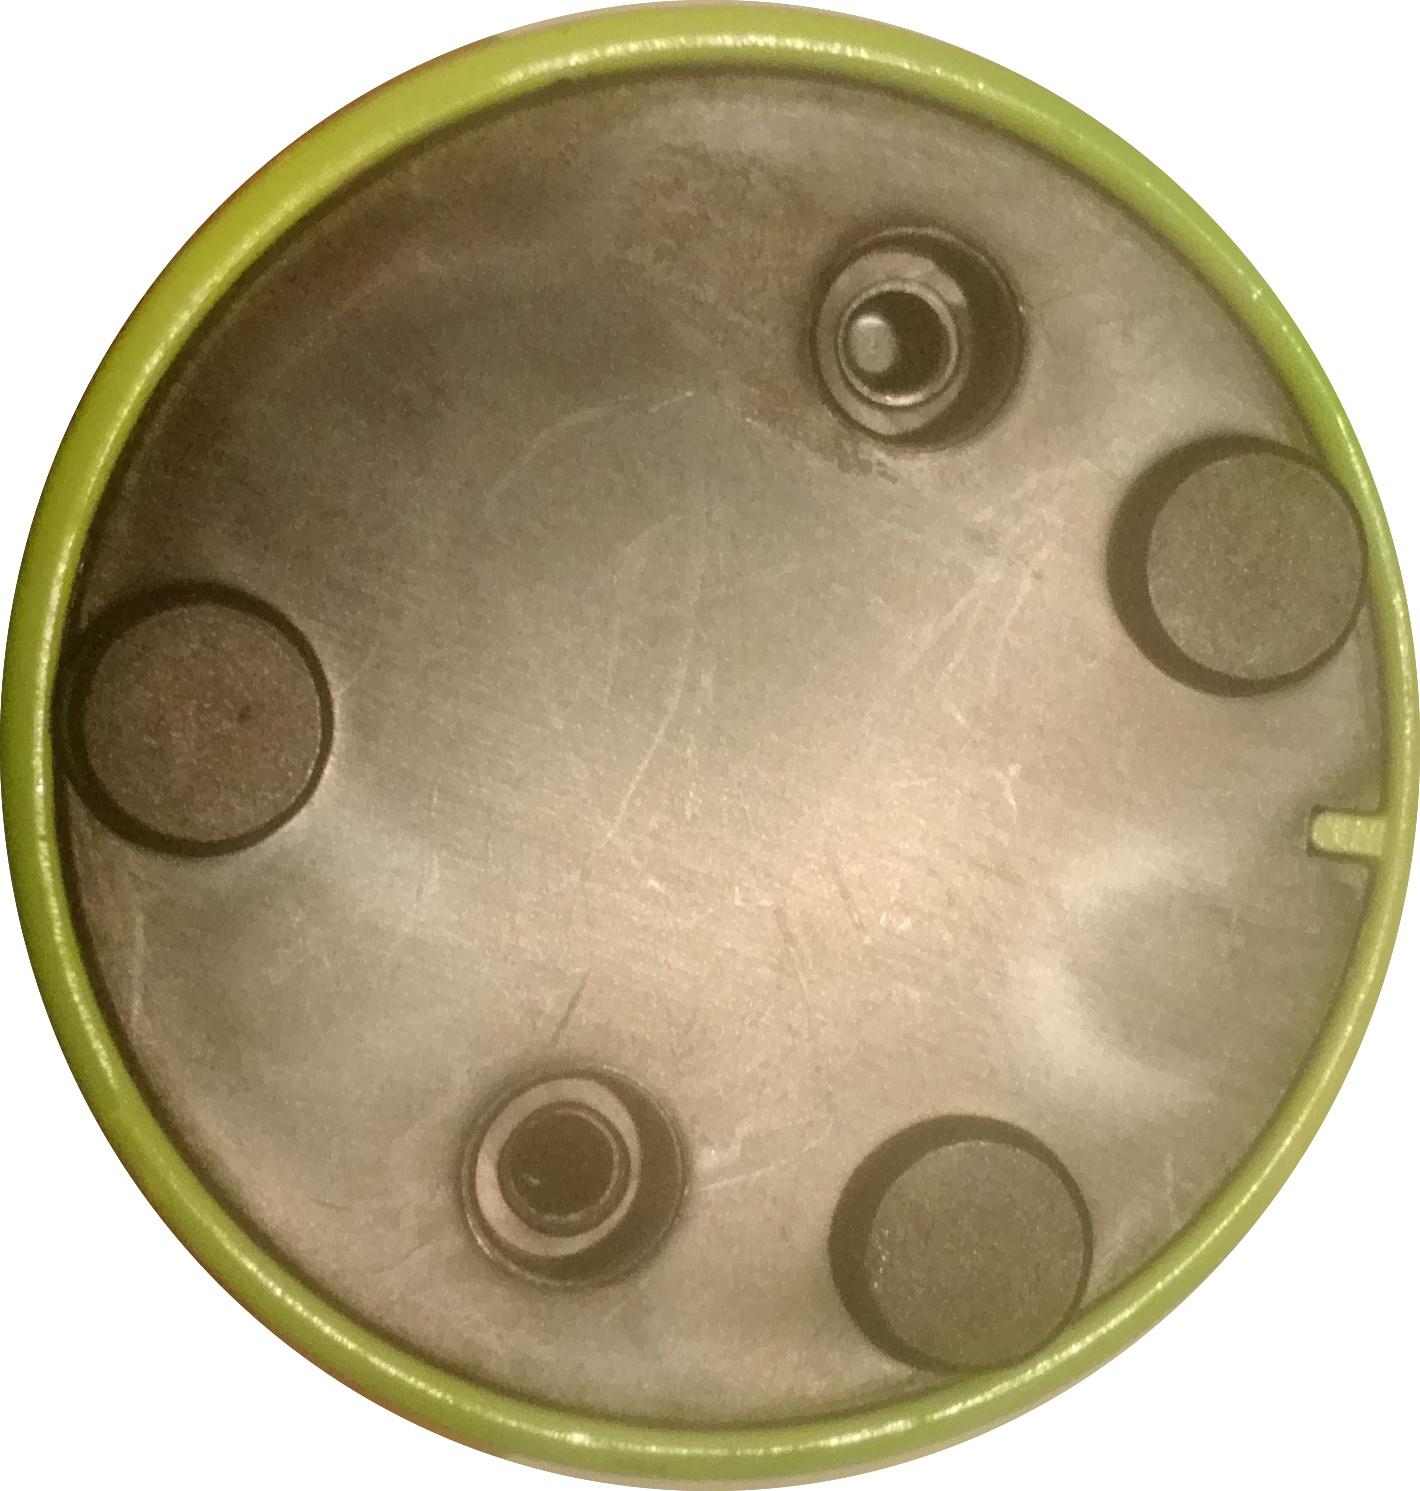
\includegraphics[width=100pt]{graphics/architecture/pieces/brassBase.png}
	\caption{Trumpet piece (frontal and base). It represents the brass family}
	\label{fig:brasspiece}
\end{figure}
\FloatBarrier

As we see in the figures above, each figure base has three little pads. These pads are used in order to determine which piece has the gamer placed on the screen. Each piece has their pads placed in a certain position. A more detailed version of the piece bases are shown below:

\begin{figure}[ht!]
	\centering
	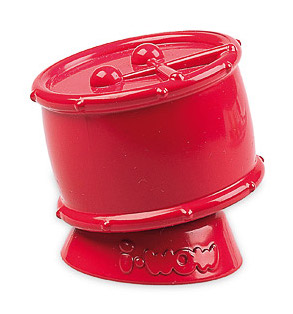
\includegraphics[width=100pt]{graphics/architecture/pieces/piecePercussion.jpg}
	\vspace{0.6cm}
	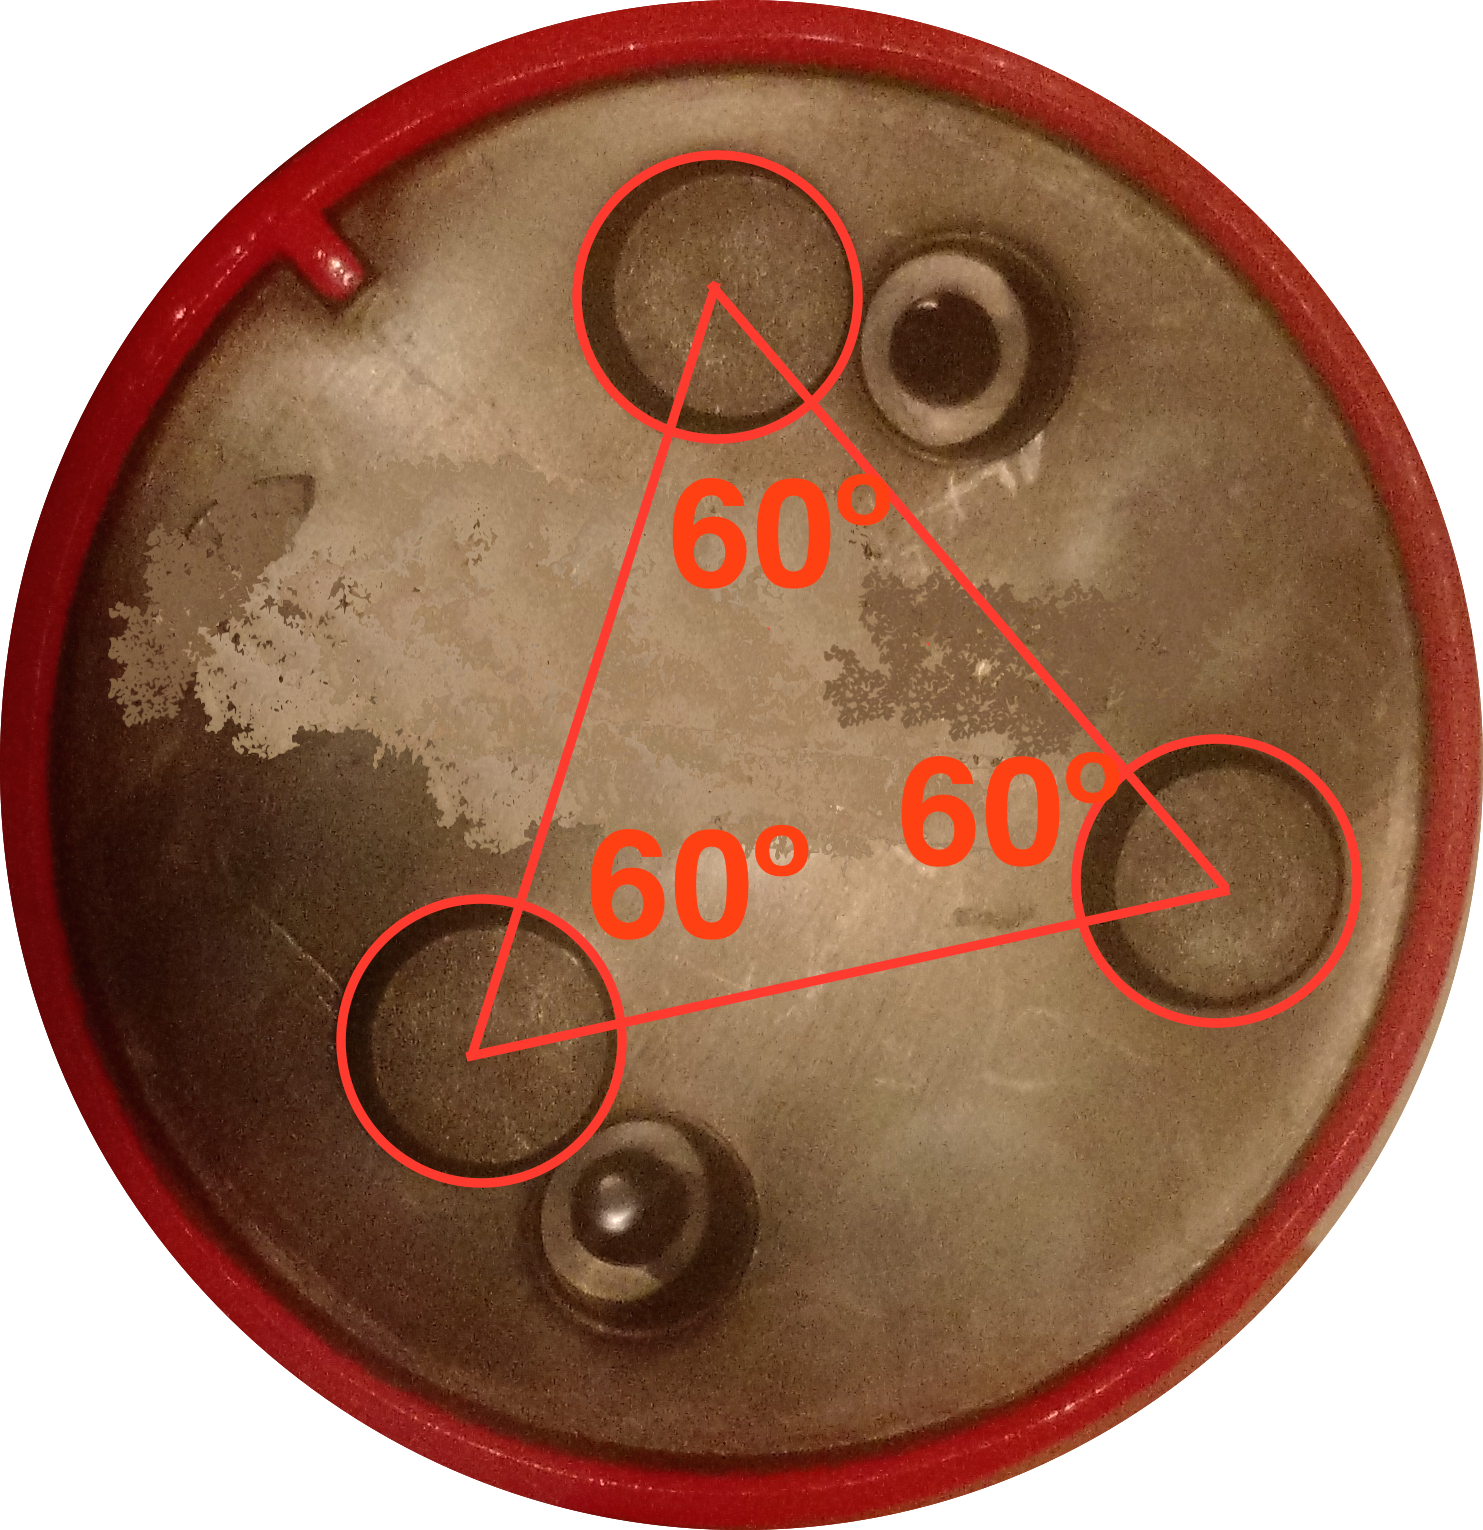
\includegraphics[width=100pt]{graphics/architecture/pieces/percussionBaseAngles.png}
	\caption{Detail of the drum base}
	\label{fig:percussionpiecedetailed}
\end{figure}

\begin{figure}[ht!]
	\centering
	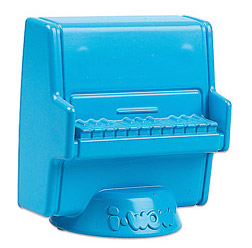
\includegraphics[width=100pt]{graphics/architecture/pieces/pieceKeyboards.jpg}
	\vspace{0.6cm}
	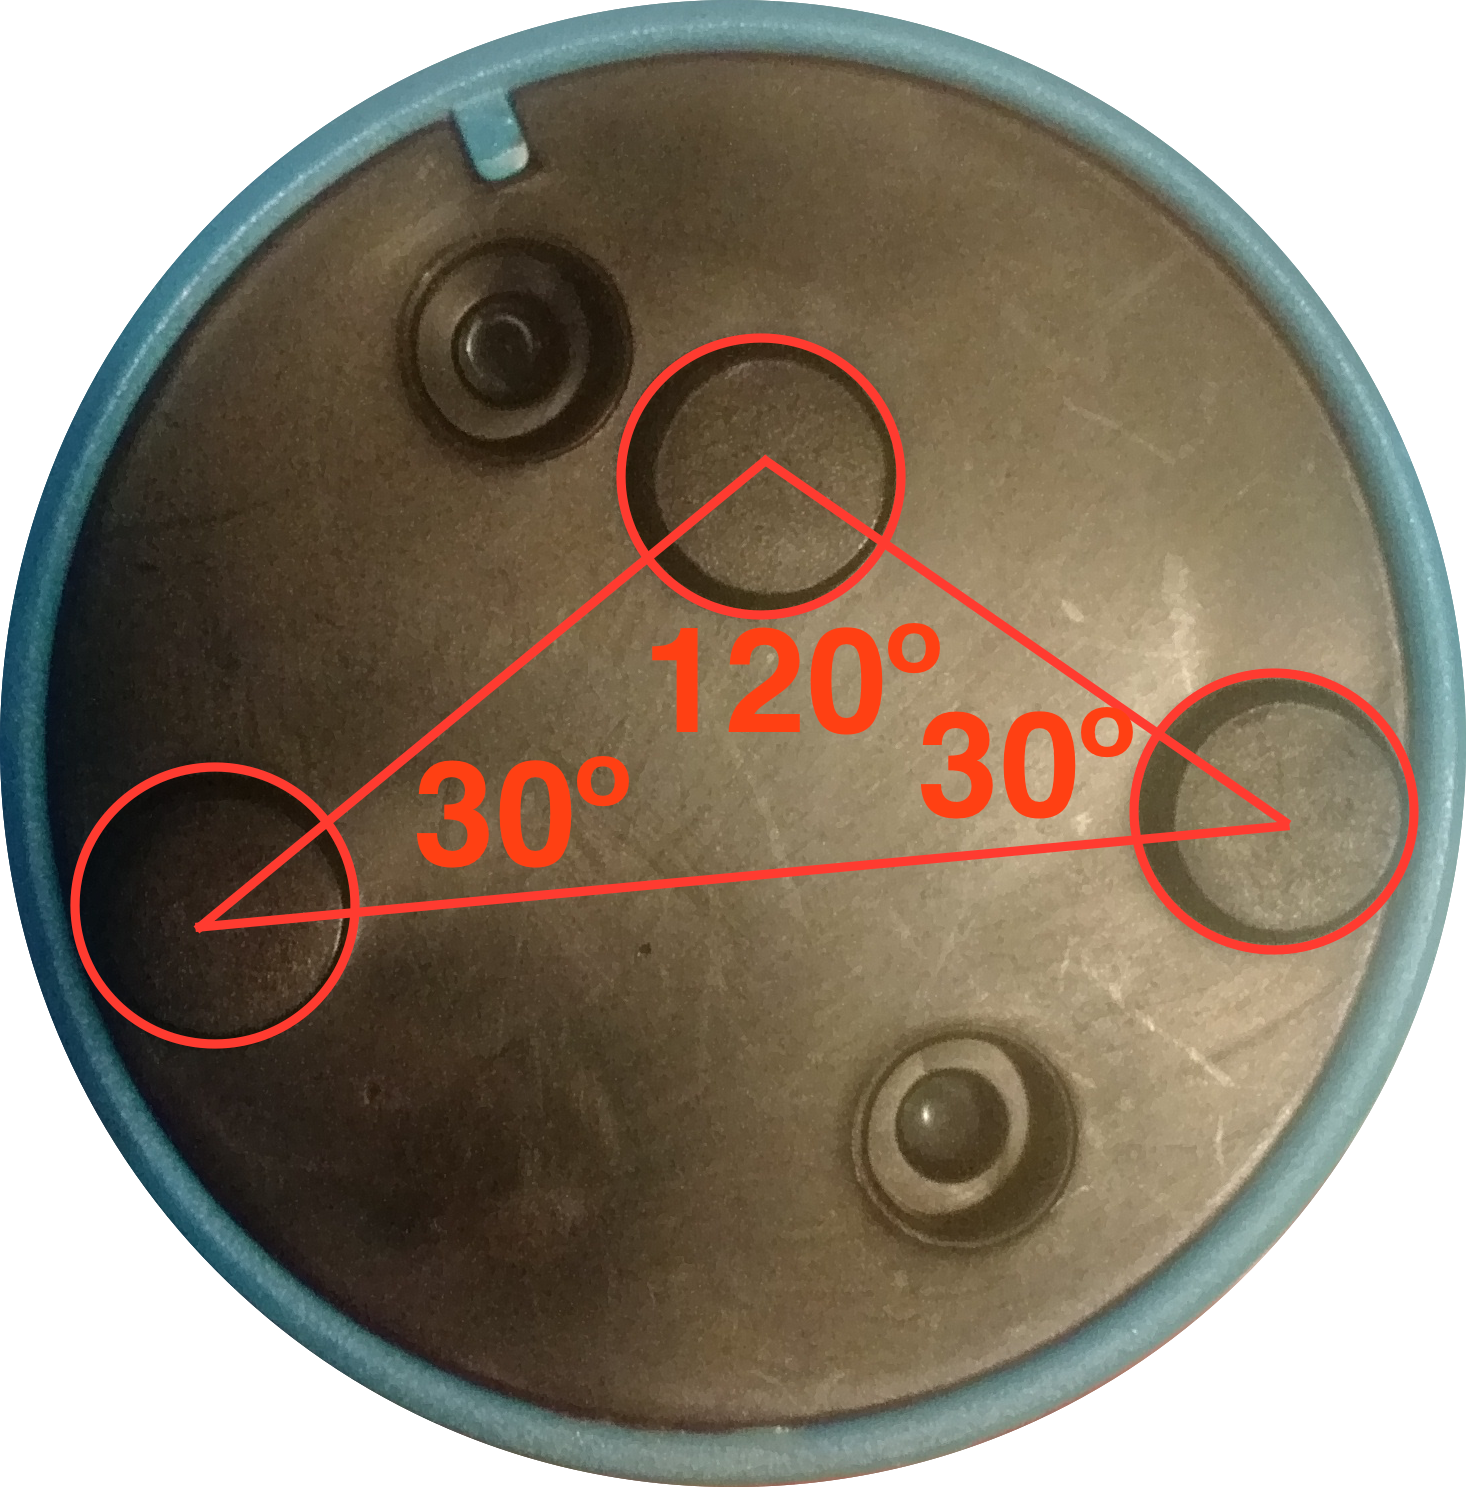
\includegraphics[width=100pt]{graphics/architecture/pieces/keyboardsBaseAngles.png}
	\caption{Detail of the piano base}
	\label{fig:keyboardspiecedetailed}
\end{figure}

\begin{figure}[ht!]
	\centering
	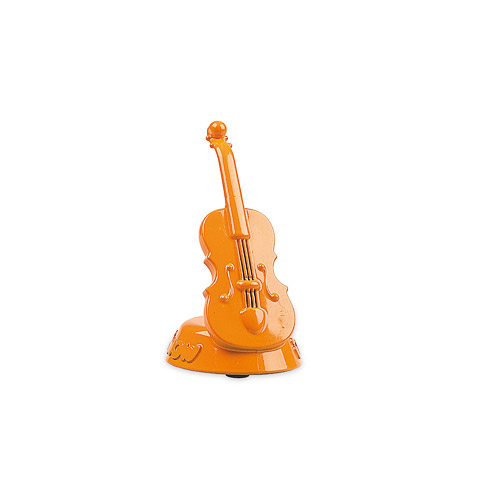
\includegraphics[width=100pt]{graphics/architecture/pieces/pieceStrings.jpg}
	\vspace{0.6cm}
	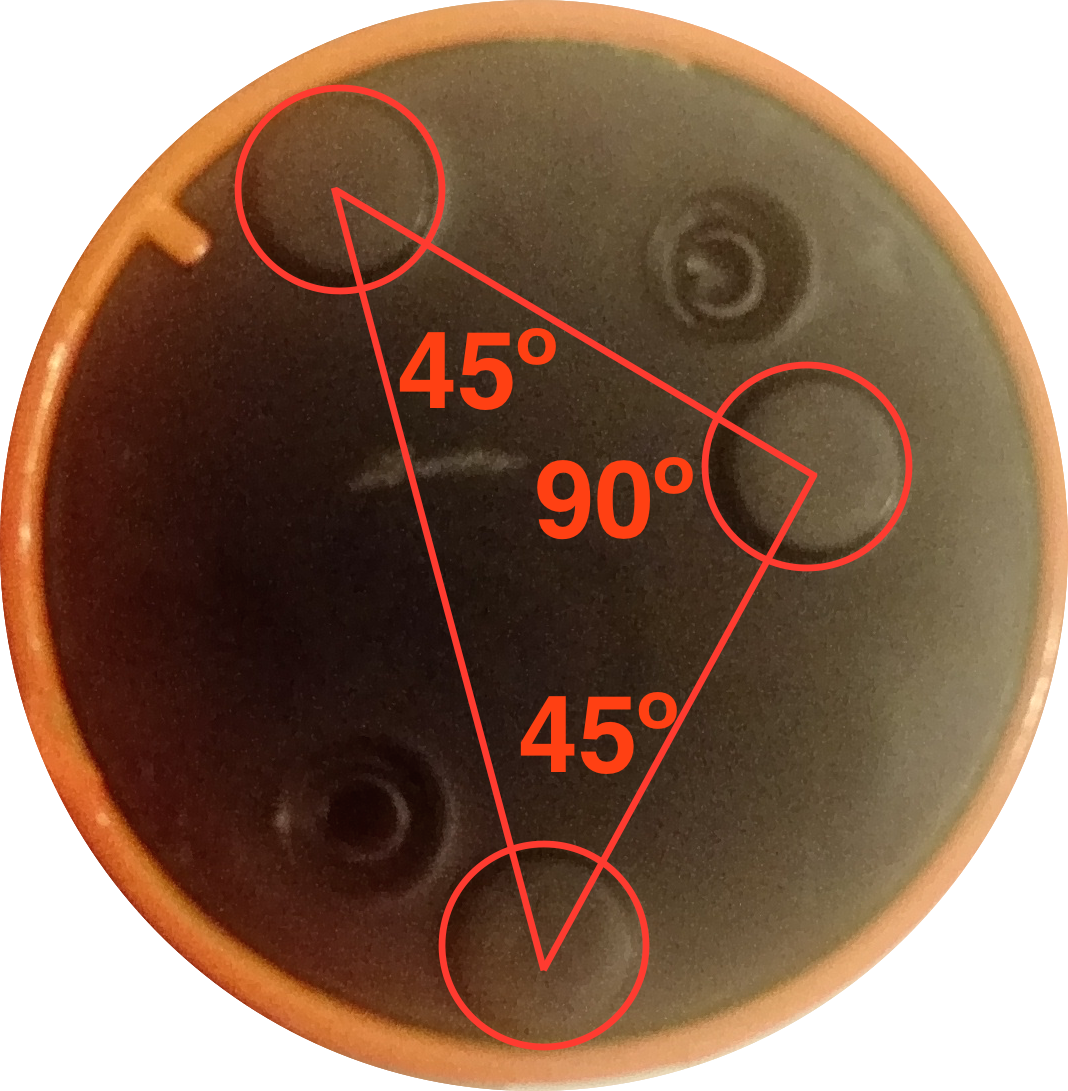
\includegraphics[width=100pt]{graphics/architecture/pieces/stringsBaseAngles.png}
	\caption{Detail of the violin base}
	\label{fig:stringspiecedetailed}
\end{figure}

\begin{figure}[ht!]
	\centering
	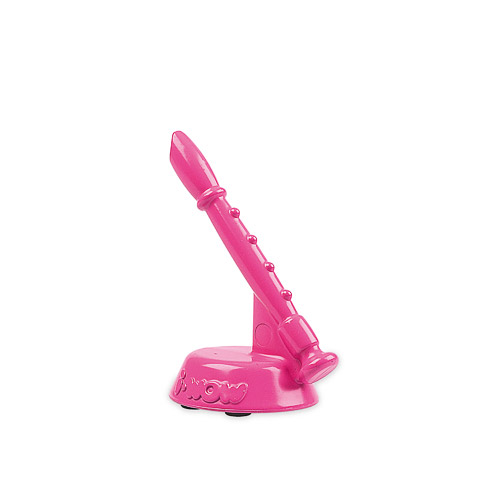
\includegraphics[width=100pt]{graphics/architecture/pieces/pieceWoodwind.jpg}
	\vspace{0.6cm}
	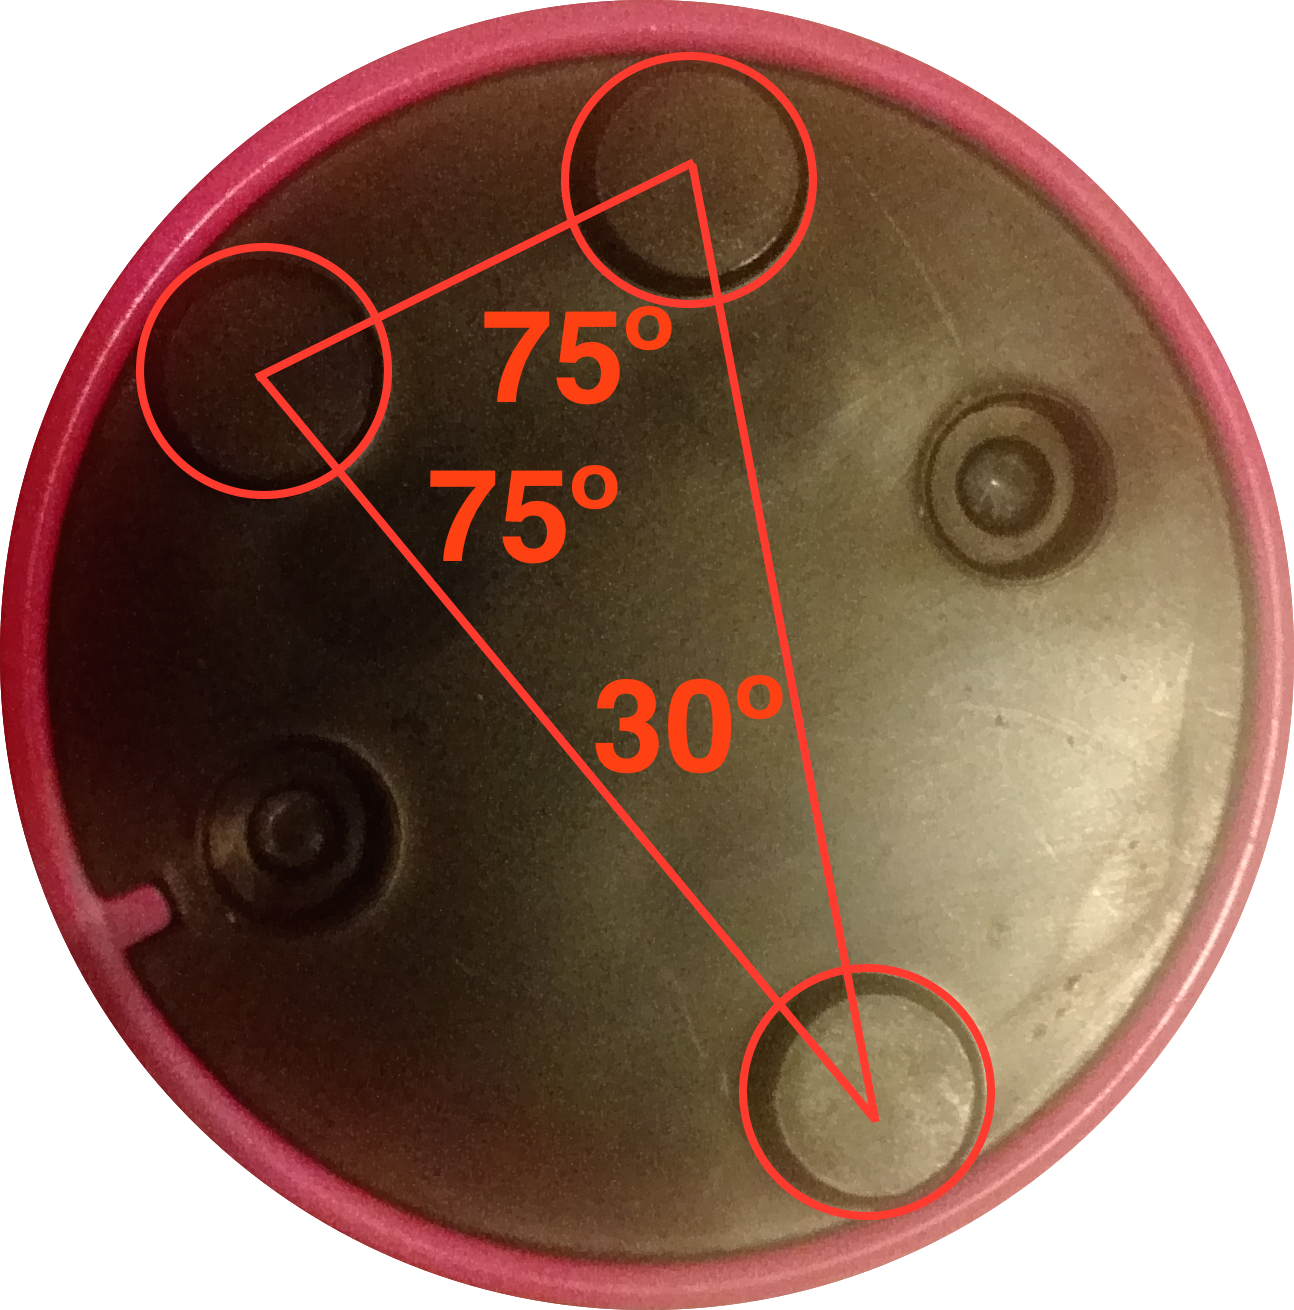
\includegraphics[width=100pt]{graphics/architecture/pieces/woodwindBaseAngles.png}
	\caption{Detail of the flute base}
	\label{fig:woodwindpiecedetailed}
\end{figure}

\begin{figure}[ht!]
	\centering
	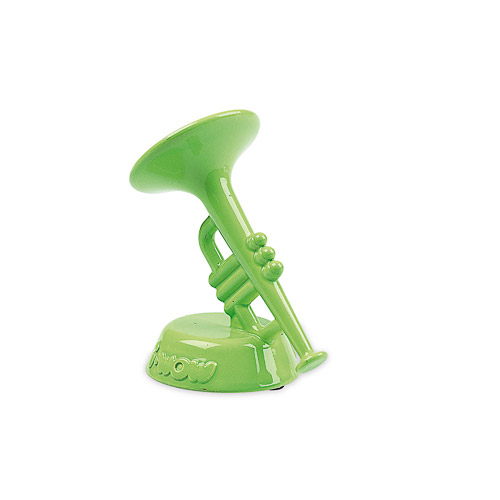
\includegraphics[width=100pt]{graphics/architecture/pieces/pieceBrass.jpg}
	\vspace{0.6cm}
	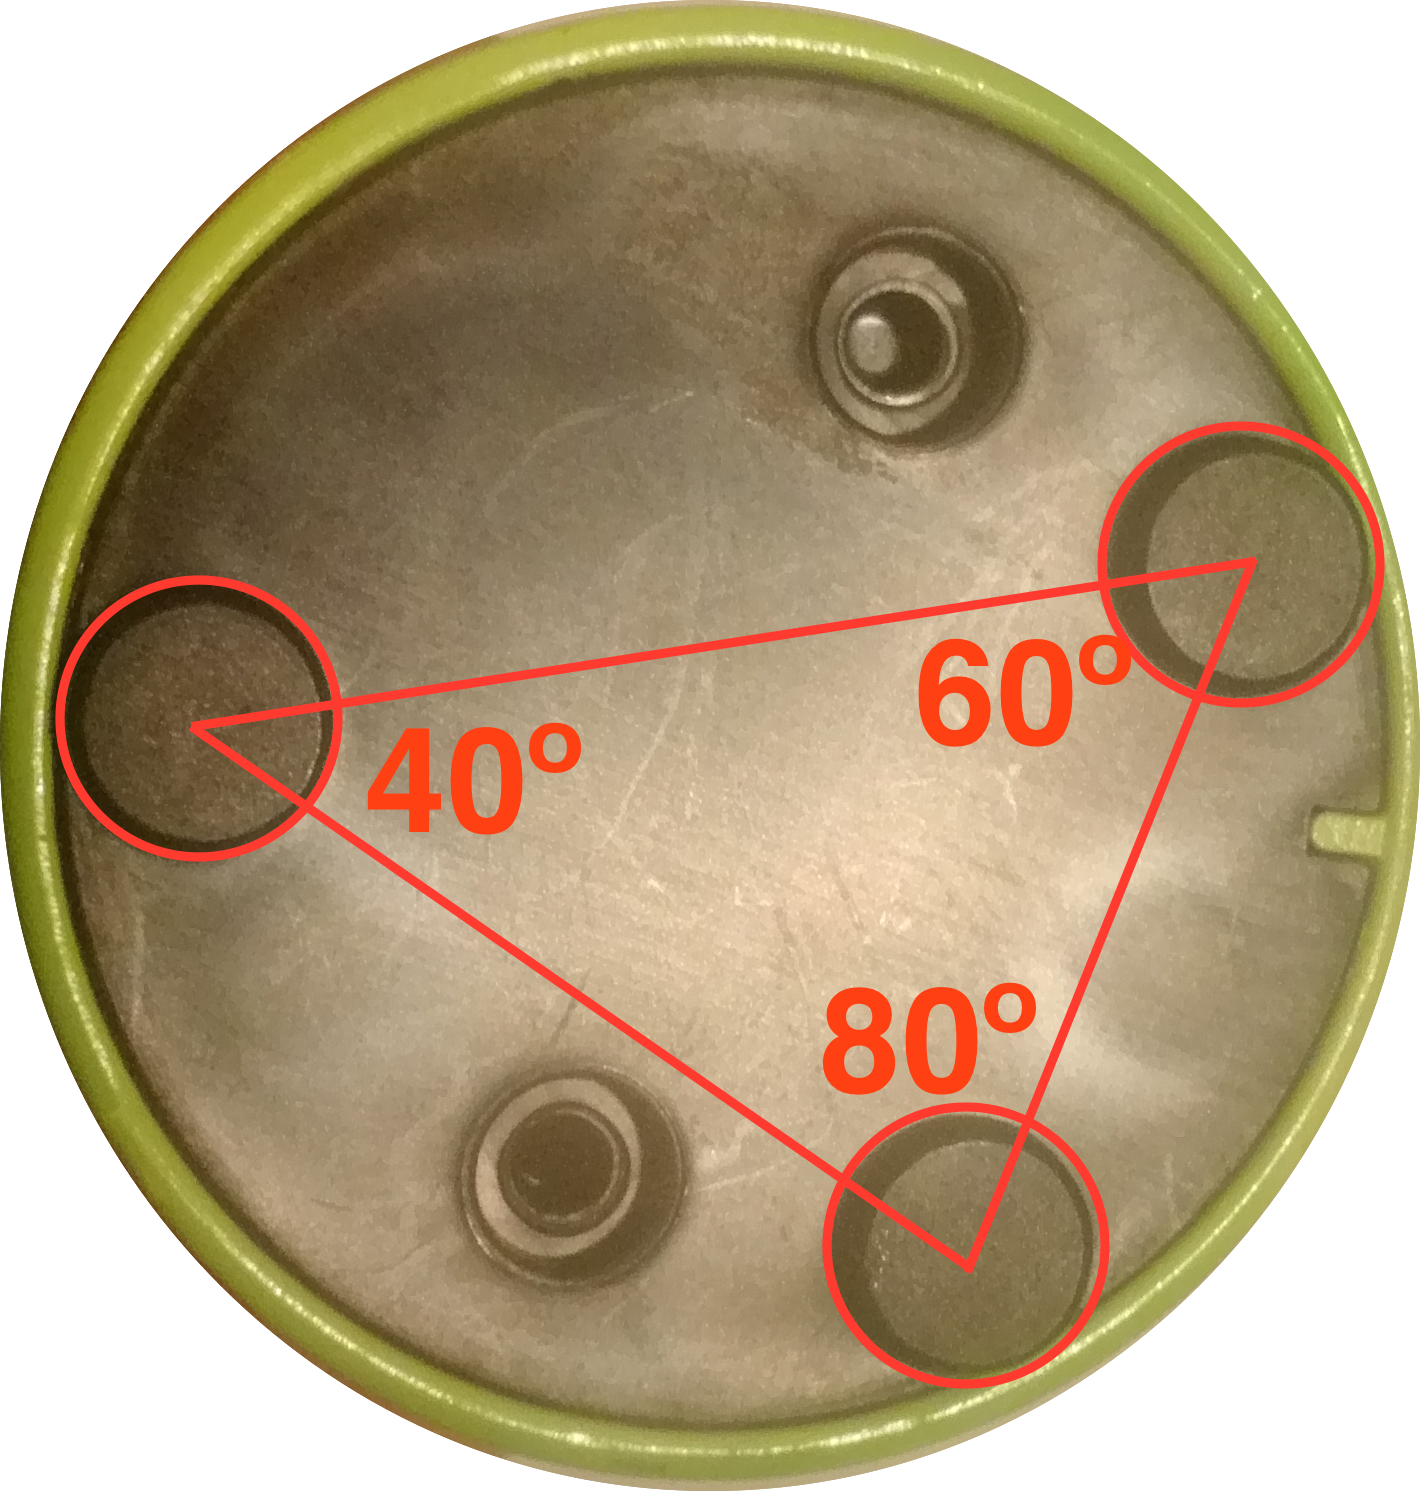
\includegraphics[width=100pt]{graphics/architecture/pieces/brassBaseAngles.png}
	\caption{Detail of the trumpet base}
	\label{fig:brasspiecedetailed}
\end{figure}
\FloatBarrier

\#Escribir sobre el algoritmo de detección

\section{Application}
\label{sec:application}
The application is the biggest module of the game. It includes the whole software development as it is shown in Figure \ref{fig:applicationarchitecture}.

\begin{figure}[ht!]
	\centering
	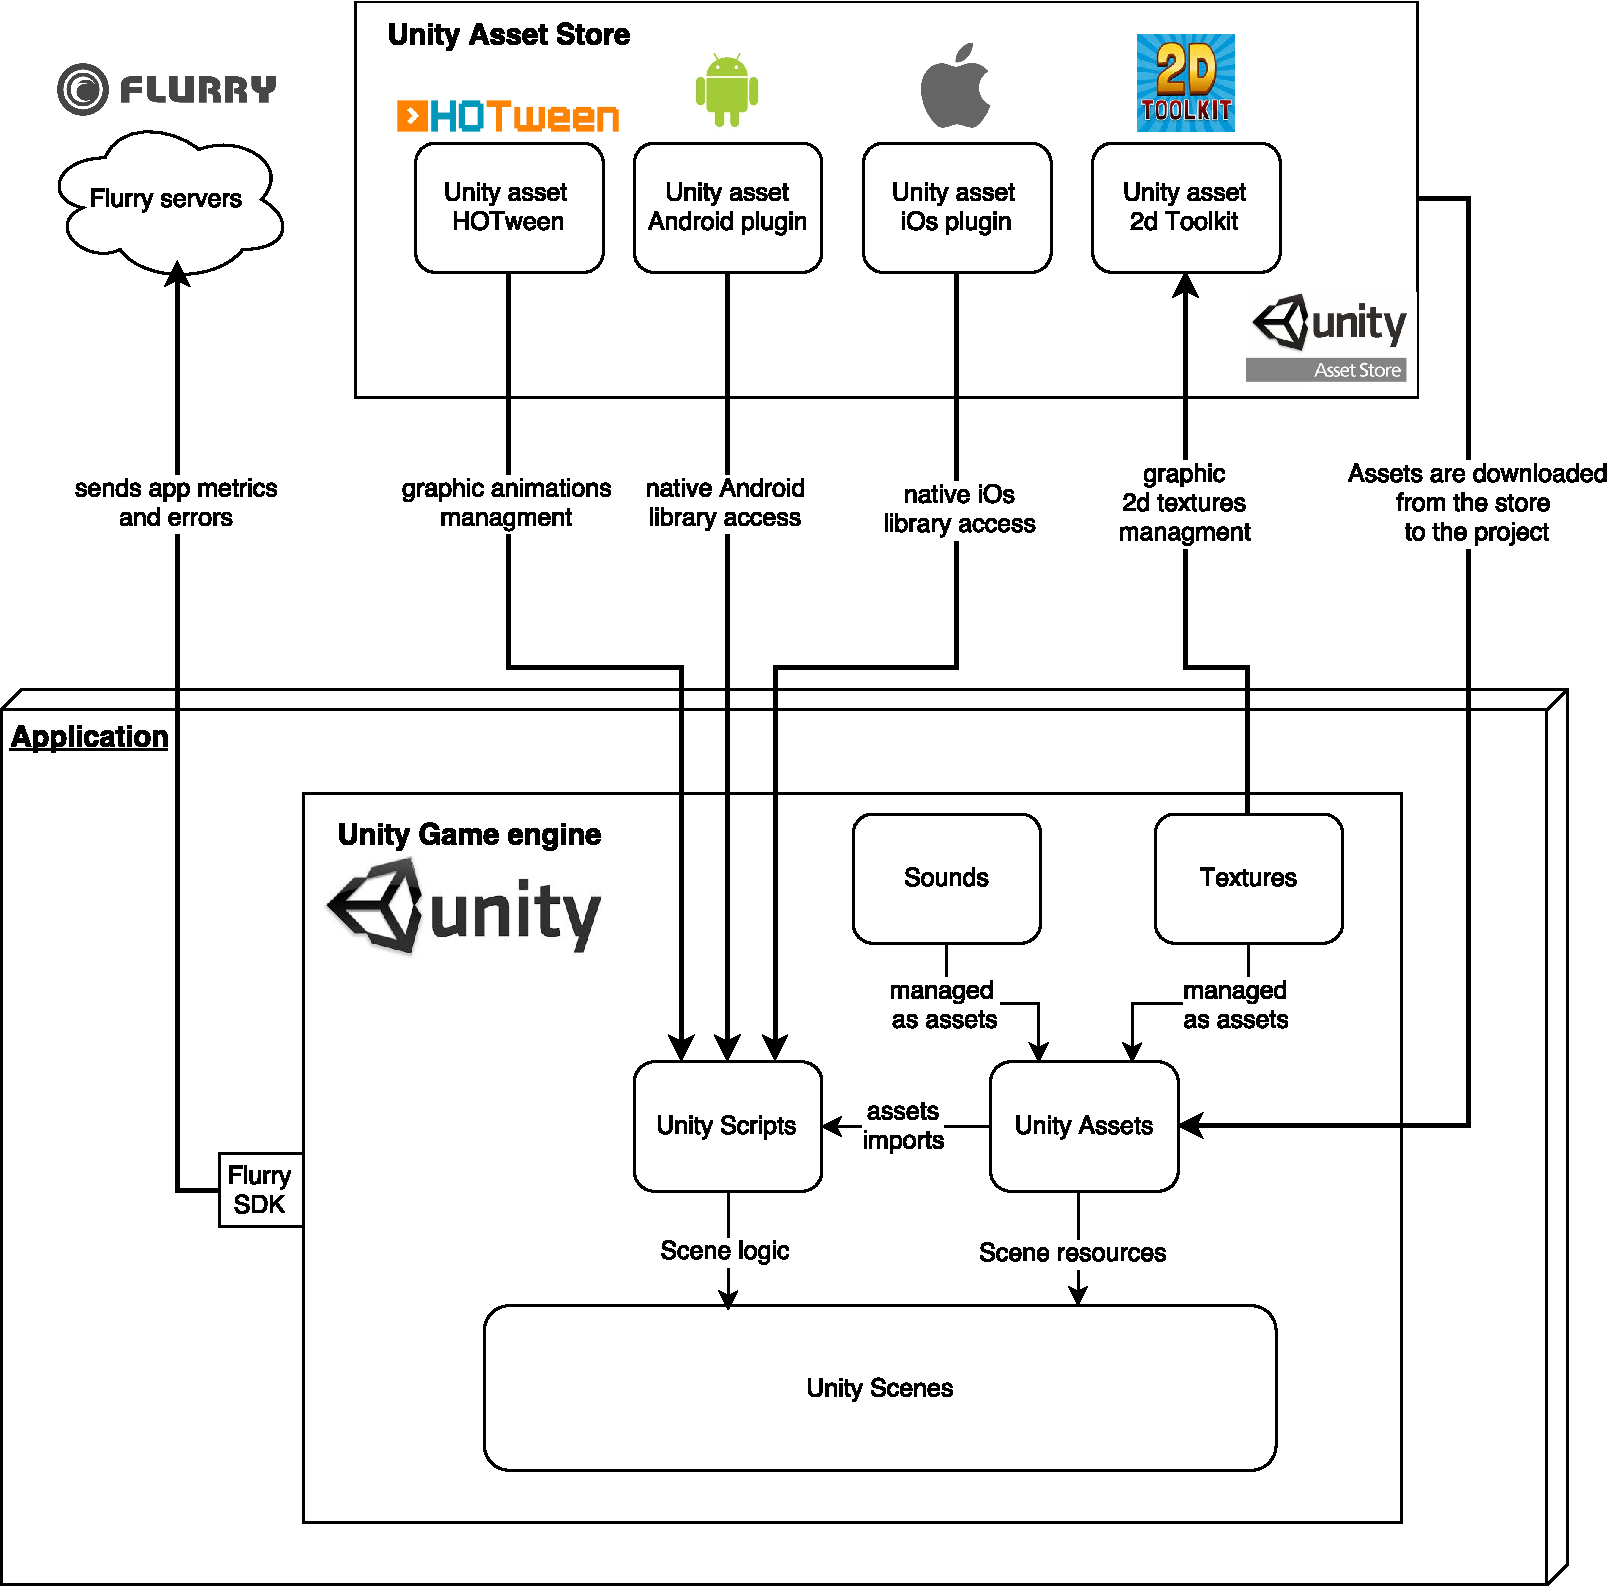
\includegraphics[width=400pt]{graphics/architecture/Application_architecture.pdf}
	\caption{Application architecture diagram}
	\label{fig:applicationarchitecture}
\end{figure}

If we look at the application architecture diagram we can see the Application module where Unity game engine will run. Unity has three main components, Unity Assets, Unity Scripts and Unity Scenes, which are described below:

\subsection{Assets}
An asset is a representation of any item that can be used in your game or project. An asset may come from a file created outside of Unity, such as a 3D model, an audio file, an image, or any of the other types of file that Unity supports. There are also some asset types that can be created within Unity, such as an Animator Controller, an Audio Mixer or a Texture Managers. In other words, assets are any resource your game uses.

Thankfully, Unity’s asset importing is robust and intelligent, it will accept all popular 3D file formats and also supports all common image file formats, including PNG, JPEG, TIFF and even layered PSD files directly from Photoshop. When it comes to audio, Unity supports WAV and AIF, ideal for sound effects, and MP3 and OGG for music.

In Figure \ref{fig:applicationarchitecture} we can see that sounds and textures are included as assets to use them, but they are not the only assets we will use. We said that there are some assets types that have been created within Unity to make development easier. In our case we will use an Animation Controller called HOTween, a 2D Texture Manager called 2dToolkit and both Android and iOs plugins. All these assets are included in our Unity project downloading them from Unity Asset Store.

The Unity Asset Store is where a growing library of free and commercial assets are placed. These assets are created both by Unity Technologies and also members of the community. A wide variety of assets is available, covering everything from textures, models and animations to whole project examples, tutorials and Editor extensions. These assets are accessed from a simple interface built into the Unity Editor and are downloaded and imported directly into your project.

Assets will be used from the Scenes and/or the Scripts, which are detailed in section \ref{subsec:unityscripts}.

\subsection{Scenes}
Scenes contain the objects of your game. They can be used to create a main menu, individual levels, and anything else. Each unique Scene file as a unique level, where you will place your environments, obstacles, and decorations, essentially designing and building your game in pieces.

We can easily make an analogy between Scenes and screens in our app. Each screen is built from a Scene where all the Assets logic are managed by the Scripts.

Creating Scenes with Unity are possible thanks to their intuitive interface, where project assets can be drag to the interface Scene and Scripts can be attached to the assets to control them.

\subsection{Scripts}
\label{subsec:unityscripts}
Scripts, known in Unity as behaviors, let you take assets in your scene and make them interactive. Multiple scripts can be attached to a single object, allowing for easy code reuse. Unity supports three different programming languages; UnityScript, C\#, and Boo. In our project we will use C\#.

As we can see in Figure 3.2, Scripts will manage Unity Assets and will use external Assets from the Unity Asset Store as libraries to make the development easier. In our case, HOTween asset allow us to automate the animation of any numeric (and some non-numeric) property or field (numbers, vectors, transforms, and so on) in many different ways. 2dToolkit provide an efficient 2D sprite, collider set-up and text system which integrates seamlessly into the Unity environment. Android and iOs plugins allow us to access to native Android and iOs libraries.

As we said, scripts will be attached to the scene assets we need to provide them the functionality we need to.


\section{Application use workflow}
The application has three game modes, for each one we will see the application use workflow to get a more precise idea of how the Gamer will interact with the application.

The three game modes were designed as a result of the Game modes use case defined in section \ref{subsec:gamemodes}:

\begin{itemize}
\item \textit{Playing instrument game mode} detailed in sub-section \ref{subsec:playinstrument_arch}.
\item \textit{Conducting orchestra game mode} detailed in sub-section \ref{subsec:conducteorchestra_arch}.
\item \textit{Discovering instrument game mode}  detailed in sub-section \ref{subsec:discoverinstrument_arch}.
\end{itemize}

\newpage
\subsection{Playing instrument game mode}
\label{subsec:playinstrument_arch}

Playing instrument game mode workflow is represented in Figure \ref{fig:playingworkflow}

\begin{figure}[ht!]
	\centering
	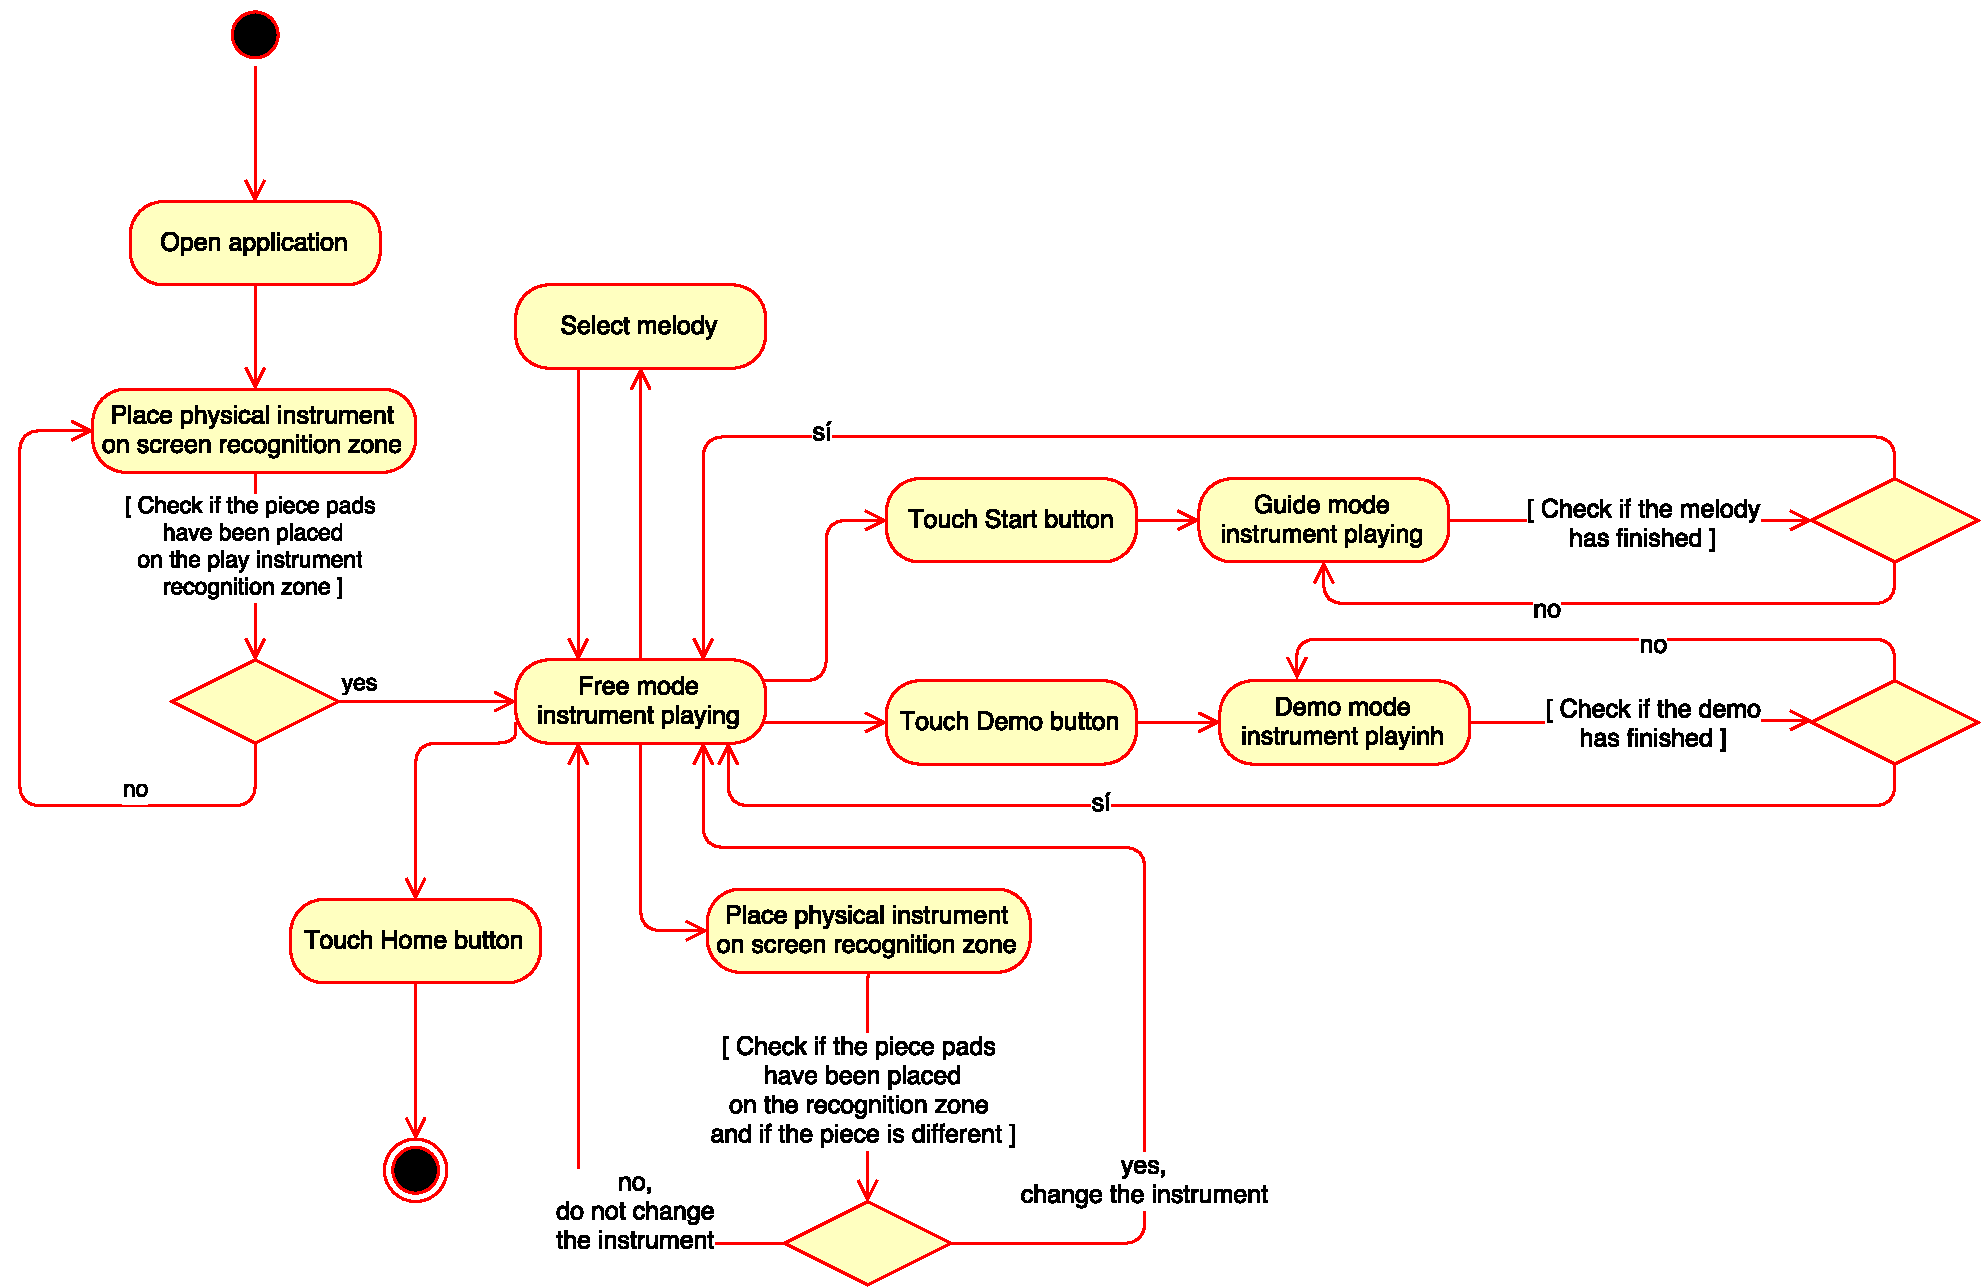
\includegraphics[width=400pt]{graphics/architecture/PlayingGameMode.pdf}
	\caption{Playing instrument game mode}
	\label{fig:playingworkflow}
\end{figure}

As we can see in Figure \ref{fig:playingworkflow}, to access \textit{Playing instrument game mode}, the gamer has to place the physical instrument miniature in the Playing mode recognition zone after opening the application. If the instrument has been placed properly, the \textit{Free mode instrument play} screen is opened.

Within this \textit{Free mode instrument play} screen, the gamer can play freely with the instrument that has been placed to access to this game mode. Also, the gamer is able to change the instrument by placing another instrument miniature on the instrument recognition zone.

The gamer has the possibility to watch a demo. After touching the demo button, the selected melody is played with the selected instrument. Also, the gamer can change the melody using the melody selector menu, that is shown after touching the melody button.

Also, the gamer can play the selected melody with the selected instrument on a \textit{guide mode instrument playing}. This guide mode is started after touching the start button. Within this guide playing, the notes are highlighted and the gamer has to play the highlighted note to compose the whole melody.

Finally, the gamer can go back to the home screen touching the home button.

\FloatBarrier

\newpage
\subsection{Conducting orchestra game mode}
\label{subsec:conducteorchestra_arch}

Conducting orchestra game mode workflow is represented in Figure \ref{fig:conductingworkflow}

\begin{figure}[ht!]
	\centering
	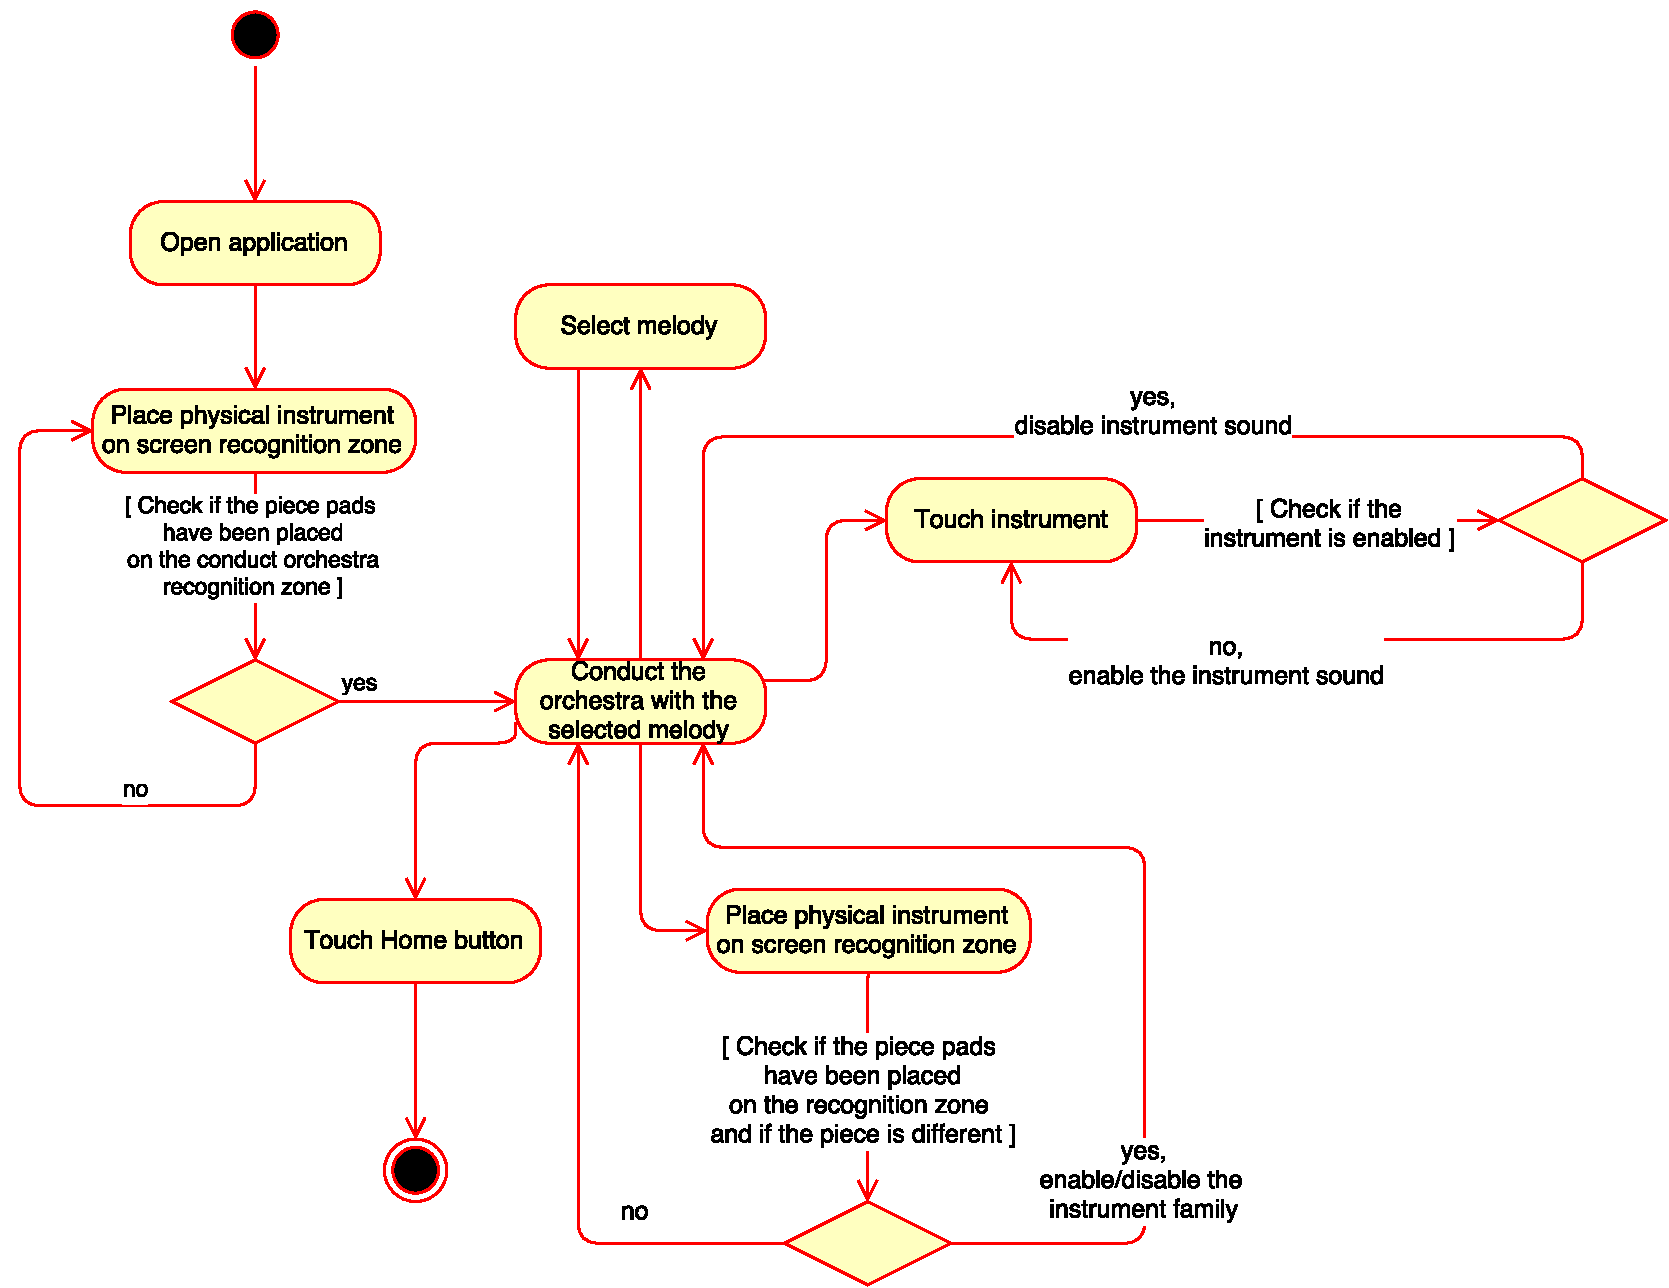
\includegraphics[width=400pt]{graphics/architecture/ConductingGameMode.pdf}
	\caption{Conducting orchestra game mode}
	\label{fig:conductingworkflow}
\end{figure}

As we can see in Figure \ref{fig:conductingworkflow}, to access \textit{Discovering instrument}, the gamer has to place the physical instrument miniature in the Discovering mode recognition zone after opening the application. If the instrument has been placed properly, the \textit{Discovering instrument} screen is opened.

Within this \textit{Discovering instrument} screen, the gamer can read information and learn about some instruments of the family instrument that has been placed to access the game mode. Also, the instrument sound can be reproduce touching the instrument sound button.

Also, the gamer is able to change the instrument by placing another instrument miniature on the instrument recognition zone.

Finally, the gamer can go back to the home screen touching the home button.

\FloatBarrier

\newpage
\subsection{Discovering instrument game mode}
\label{subsec:discoverinstrument_arch}

Discovering instrument game mode workflow is represented in Figure \ref{fig:discoveringworkflow}

\begin{figure}[ht!]
	\centering
	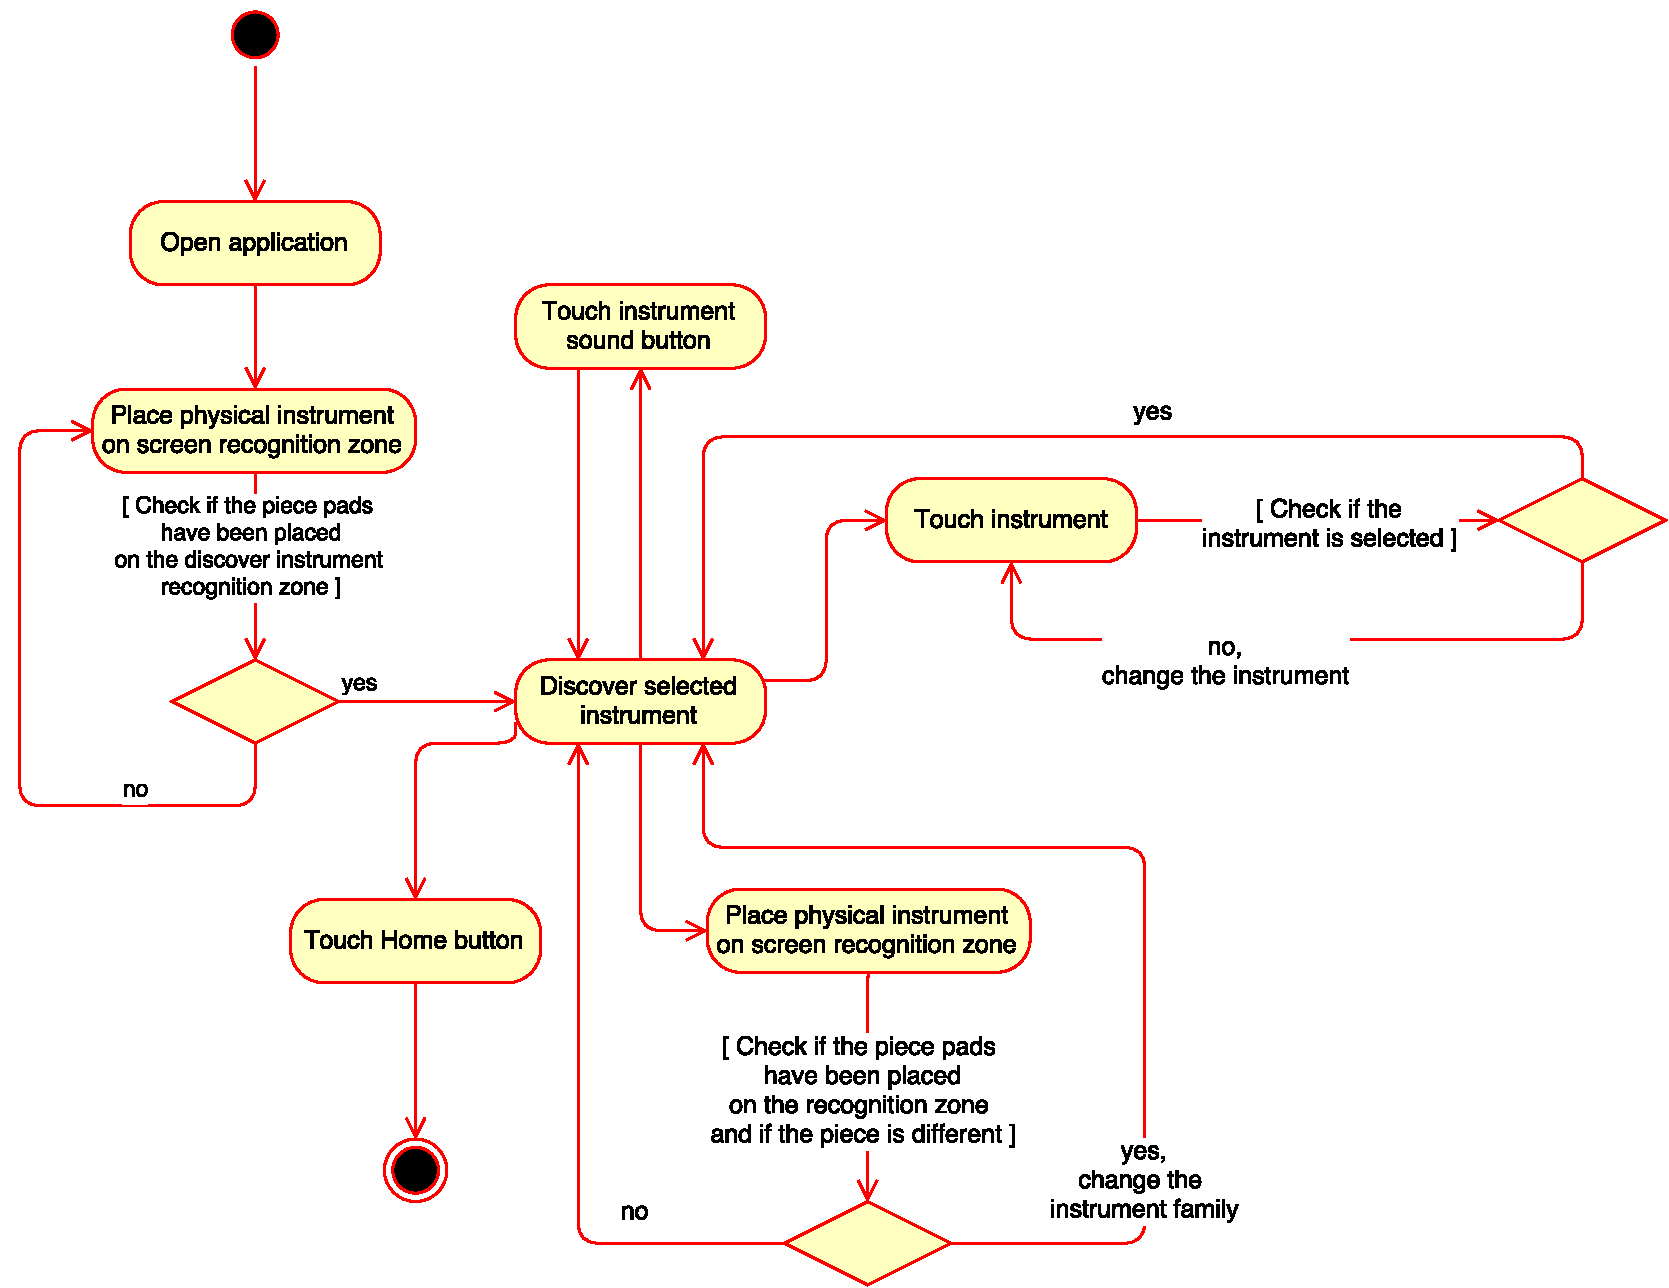
\includegraphics[width=400pt]{graphics/architecture/DiscoveringGameMode.pdf}
	\caption{Discovering instrument game mode}
	\label{fig:discoveringworkflow}
\end{figure}

As we can see in Figure \ref{fig:conductingworkflow}, to access \textit{Conducting the orchestra}, the gamer has to place the physical instrument miniature in the Conducting mode recognition zone after opening the application. If the instrument has been placed properly, the \textit{Conducting orchestra} screen is opened.

Within this \textit{Conducting orchestra} screen, the gamer can conduct an orchestra which is playing the selected melody. This melody can be changed by the gamer using the melody selector menu, that is shown after touching the melody button.

When this game mode is opened, the melody start to be played with all the instrument enabled. The gamer is able to enable or disable an instrument sound. Also, the gamer can enable or disable an entire family instrument placing one of the physical instrument miniatures in the instrument recognition zone.

\FloatBarrier

\section{Conclusions}

\chapter{Case study}

\begin{chapterintro}
In this chapter we are going to describe two selected use cases that represents how the gamer will interact with the application.
Firstly, we will describe the gamer interaction with the playing instrument game mode. Secondly, we will study the conduct orchestra game mode 
\end{chapterintro}

\cleardoublepage

\section{Introduction}

In both use cases, two actors are involved, the gamer and the instrument recognition algorithm.

\begin{table}[!htpb]
\centering
\begin{tabular}{|c|c|x{6cm}|}
\noalign{\hrule height 2pt}
\textbf{Actor identifier} & \textbf{Role} & \textbf{Description}\tn
\hline
ACT-1 & Gamer & End user that plays the game using the physical instruments and the application\tn
\hline
ACT-2 & Instrument recognition algorithm & Algorithm that detects what physical figure has been placed on the application recognition zones\tn
\noalign{\hrule height 2pt}
\end{tabular}
\caption{Actors list}
\label{tab:actoresusecase}
\end{table}

In the following sections we will explain two of the principal application game modes:

\begin{itemize}
\item \textit{Playing instrument game mode} detailed in section \ref{sec:playinginstrumentgm}.
\item \textit{Conducting orchestra game mode} detailed in section \ref{sec:conductingorchestragm}.
\end{itemize}

The \textit{Gamer} is able to access to both game modes from the application home screen, using one of the physical instrument miniature. Within each game mode, the gamer is able to interact with every component in order to select other musical instrument, change melodies, play an instrument, watch a play instrument demo, choose what instruments must be playing, etc.

The \textit{Instrument recognition algorithm} allows the application engine to detect which physical instrument miniature has been placed on the screen recognition zones. As a result, the gamer is able to interact with the game mode using the physical instrument miniatures.

\newpage
\section{Playing instrument game mode}
\label{sec:playinginstrumentgm}

Playing instrument game mode

\newpage
\section{Conducting orchestra game mode}
\label{sec:conductingorchestragm}

Conducting orchestra game mode

\newpage
\section{Conclusions}


\chapter{Conclusions and future lines}
\label{chap:conclusions}
\begin{chapterintro}
In this chapter we will describe the conclusions extracted from this master thesis, the achievements and thinkings about future work.
\end{chapterintro}

\cleardoublepage
\section{Conclusions}

By fetching existing services and widgets on the Internet, we have created a powerful search engine without having any own content, enabling final user find those services that he needs, that is part of the mash-up generation philosophy.

This project has been developed in the scope of an European FP7 project contributing to the automated discovery section. This helped us to solve problems that without being part of a big problem we would not have noticed, like taking into account that final endpoint servers are not going to be as powerful as developing ones or making the system scalable.

Also helped to extend functionalities of other projects, such as Episteme.

We have used existing technologies whenever it was possible, and this helped improving them when more complex requisites where necessary. As an example, this happened with Scrappy, which was modified, created a branch and then merged again with extra functionalities.

Dividing the project into different modules forced us to rely on existing web and software standards which helped us to integrate and interconnect all of them.

We experienced big changes as early technology adopters, such as new versions of the SPARQL language fixing bugs and creating new functionalities. We have dared to use extremely new technologies still in alpha developments, with its pros and cons.

\section{Achieved goals}

\begin{description}
\item[Fetch content automatically]
This goal has been achieved successfully. We have been able to discover existing content from websites and then fetch it. This helped us to have a big repository of services and content that the user will need. This is deeply described in chapter \ref{sec:scrappy}.

\item[Structure content] It was essential to structure the content fetched from the Internet. This has been possible thanks to semantic and linked data technologies. This is detailed in chapter \ref{subsec:limonontology}

\item[Store content] An other crucial feature that was successfully implemented was how to store all the information without losing the structured format described before. This has been achieved by using semantic repositories. More information can be consulted in chapter \ref{sec:omrsesame}.

\item[Rank content]The content without knowing if it is useful or not is useless. One of the main goals was to make possible to distinguish good and bad discovered content. This has been achieved by defining and implementing algorithms that will automatically rank the stored content. The algorithm and it's implementation is explained in chapter ref{sec:rankingmodule}.
 
\item[Manage content] It was completely necessary to manage and administer the discovered content by the administrator user. This has been achieved by creating an interface that allows searching and filtering into the automated discovered content and after selecting the useful content. This is described in chapter \ref{sec:omradmin}.

\item[Search content] The main goal of the project was enabling the user search the services he needed. This has been done by creating an easy-to-use interface that queries the repository and lets the user find suitable services. To see detailed information see chapter \ref{sec:omrclientbrowser}.

\item[Suggest similar content] Many times the user does not know what he wants, an other important role of the project was suggesting the user possible results that matches his needs. This has been achieved by using semantic search empowered technologies. Nevertheless, this has been implemented in a simpler scenario using different content and different ontology. This feature is available in the Job Matching demo\footnote{http://demos.gsi.dit.upm.es/job-matching/}.

\end{description}

\section{Future work}

There are several lines than can be followed to continue and extend features of this work.

In the following points some fields of study or improvement are presented to continue the development.

\begin{itemize}
	\item In automated discovery enable only search for new services. Without scrapping the entire web again we would gain a lot if processing time and this could make possible more frequent discoveries and more up to date content.
	\item Also fetching services and widgets from new Internet repositories.
	\item Not only fetch content from existing repositories, explore the web to discover new ones. This makes possible to have different content and always new and undiscovered services.
	\item Make the discovering service to be launched from web interface. Now it is launched from console. Integrated into the administrative interface would be optimal.
	\item Make discovery date visible. This would make possible to know if the information about a service is reliable. Also making possible to update information of only selected services.
	\item New ways of ranking content, based on social networks and popularity on the Internet.
	\item Categorize widgets and services for existing platforms. For example Wordpress\footnote{http://wordpress.org/} plugins.
	\item Discover mobile services. Content discovered right now is desktop oriented.
	\item Let the user try and show a demonstration of the services and widgets in the search interface.
	\item Semantic search and suggestions to find similar content that could fit in the user's preferences. This has been already done in a smaller scenario as a proof of concept.

\end{itemize}



\appendix
\cleardoublepage
\chapter{Application game screens}
\label{apdx:gamescreens}

This appendix shows all the screens which conform the application. It goes through the three different game modes and shows all the screens contained within them.

\cleardoublepage

\section{Home}

\begin{figure}[ht!]
  \centering
  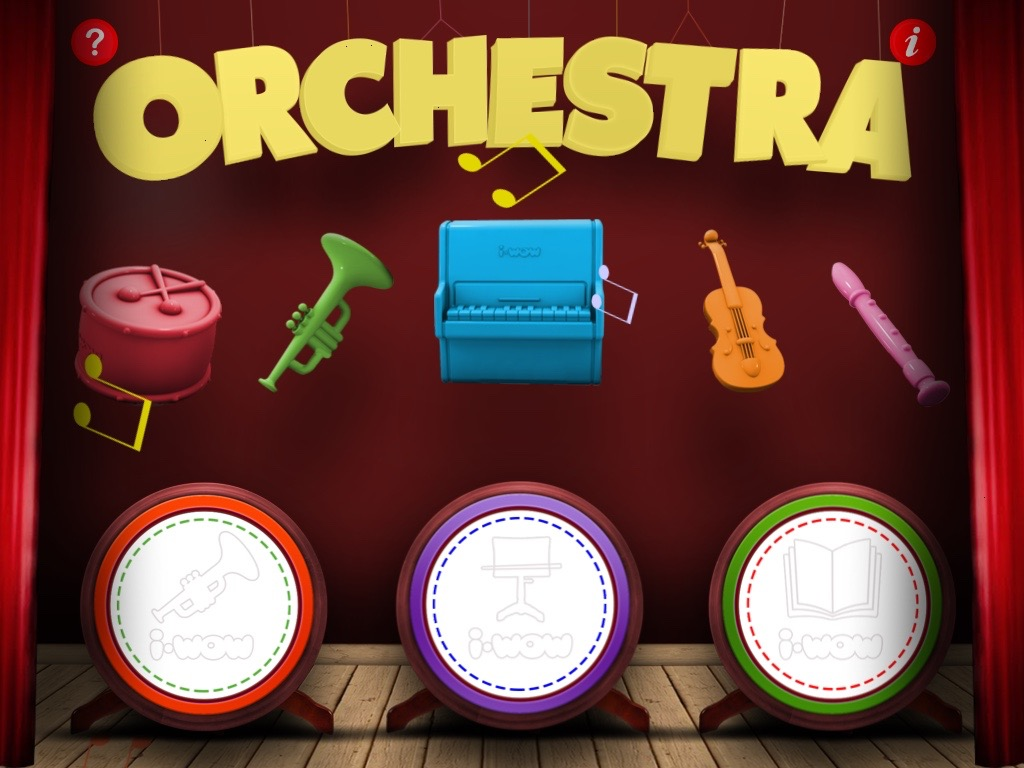
\includegraphics[width=350pt]{graphics/use-case/home_screen.jpg}
  \vspace{0.05cm}
  \caption{Application Home Screen}
  \label{fig:home_screen}
  \vspace{0.6cm}

  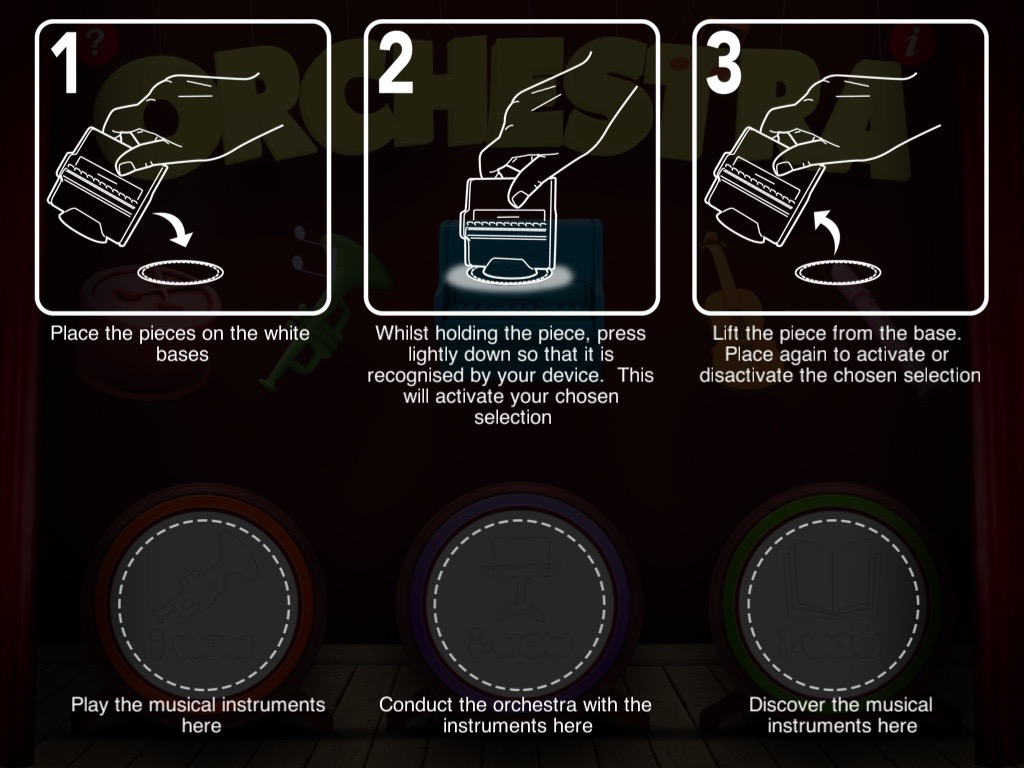
\includegraphics[width=350pt]{graphics/use-case/help_home_screen.jpg}
  \vspace{0.05cm}
  \caption{Help Home Screen}
  \label{fig:help_home_screen}
\end{figure}

\section{Playing game mode}

\begin{figure}[ht!]
  \centering
  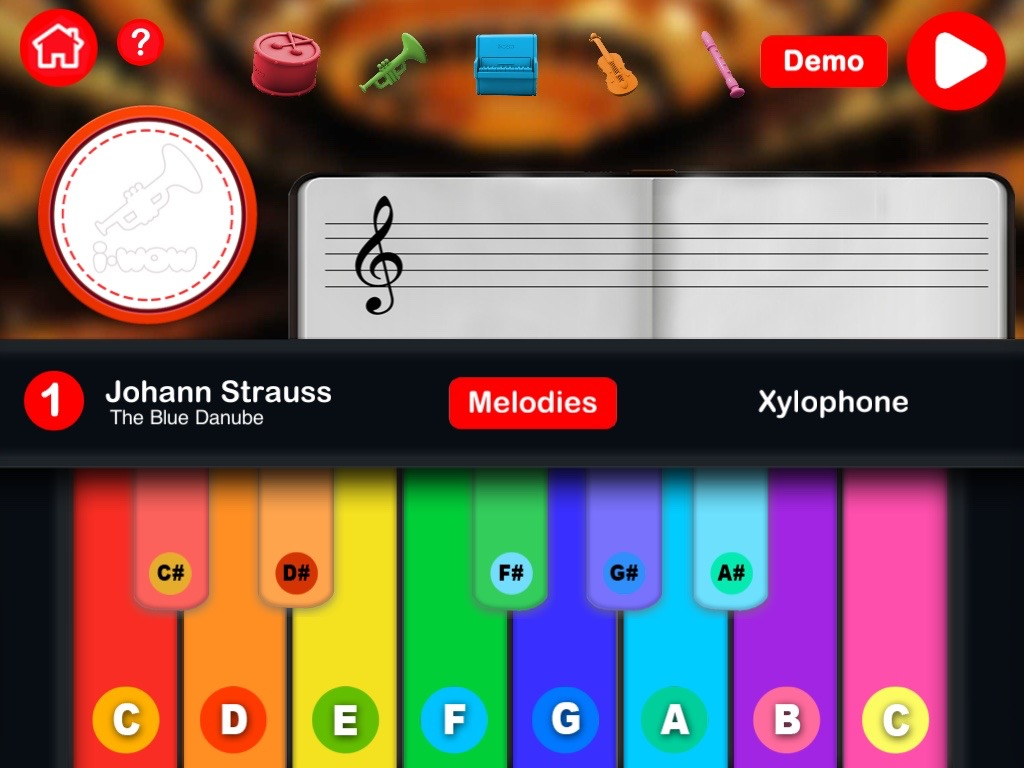
\includegraphics[width=350pt]{graphics/use-case/playing_xylo_start_screen.jpg}
  \vspace{0.05cm}
  \caption{Xylophone playing instrument game mode}
  \label{fig:playing_xylo_start_screen}
  \vspace{0.6cm}

  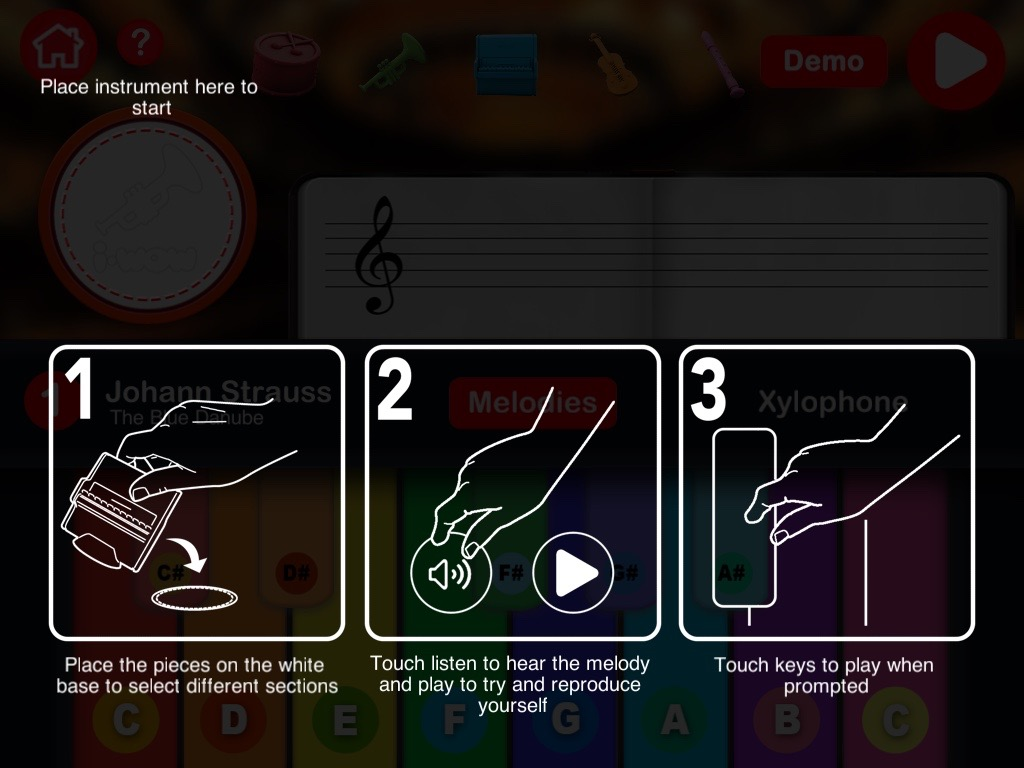
\includegraphics[width=350pt]{graphics/use-case/help_playing_screen.jpg}
  \vspace{0.05cm}
  \caption{Help information playing instrument game mode}
  \label{fig:help_playing_screen}
\end{figure}

\begin{figure}[ht!]
  \centering
  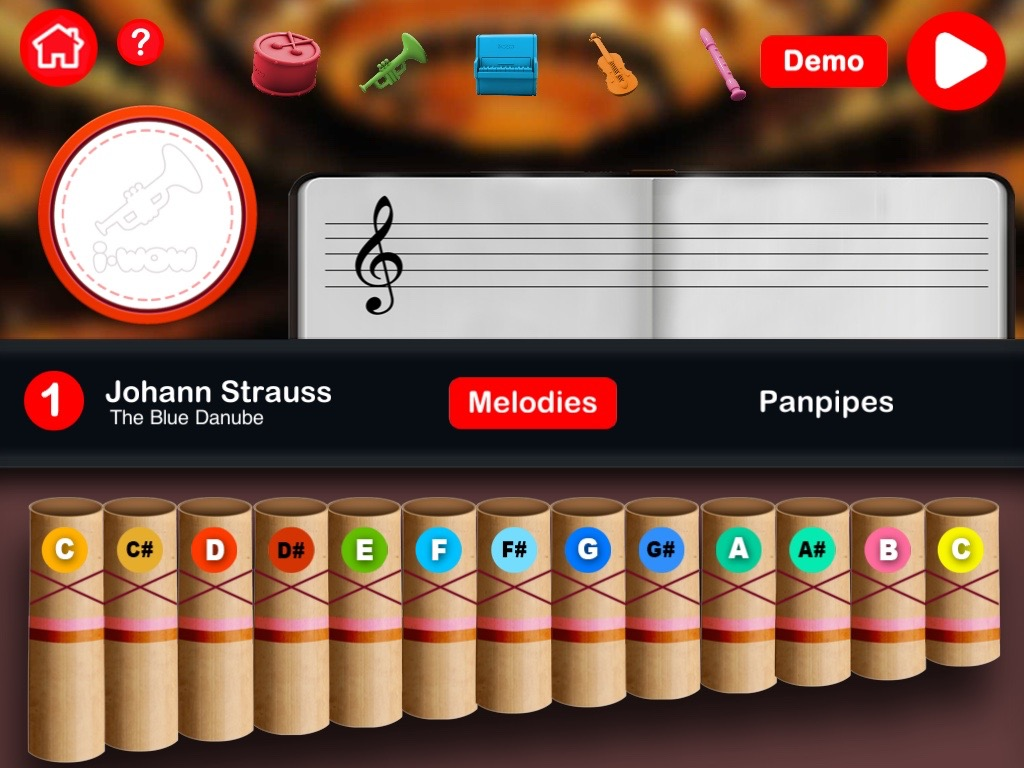
\includegraphics[width=350pt]{graphics/use-case/playing_panpipes_screen.jpg}
  \vspace{0.05cm}
  \caption{Playing panpipes screen}
  \label{fig:playing_panpipes_screen}
  \vspace{0.6cm}

  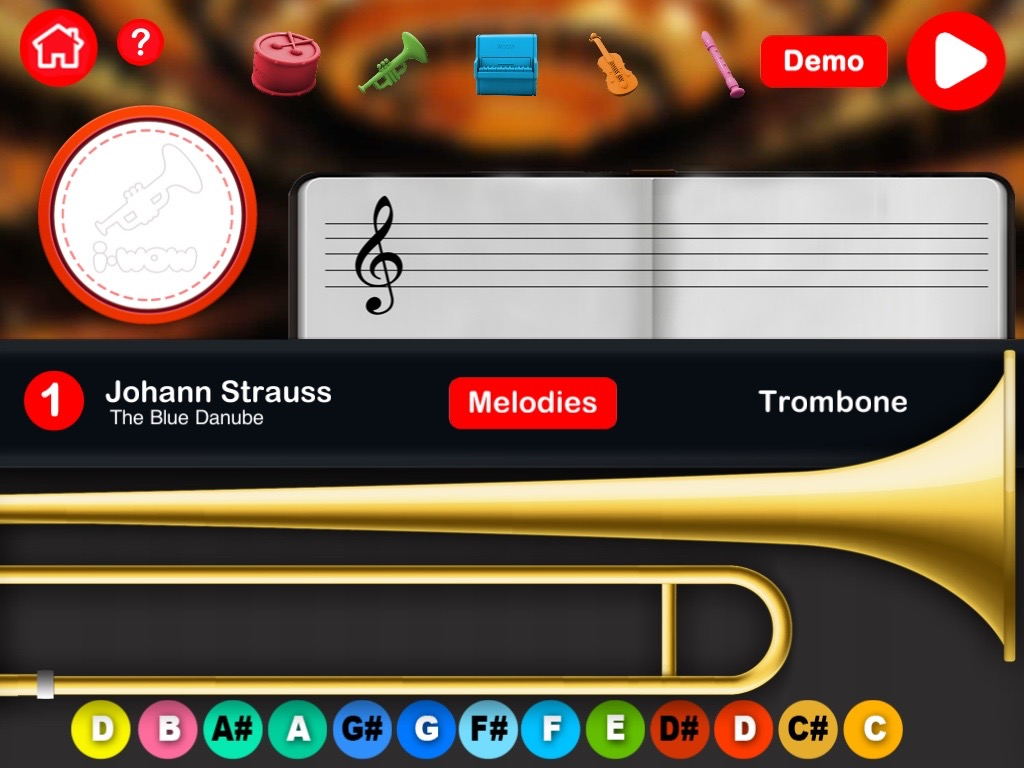
\includegraphics[width=350pt]{graphics/use-case/playing_trombone_screen.jpg}
  \vspace{0.05cm}
  \caption{Playing trombone screen}
  \label{fig:playing_trombone_screen}
\end{figure}

\begin{figure}[ht!]
  \centering
  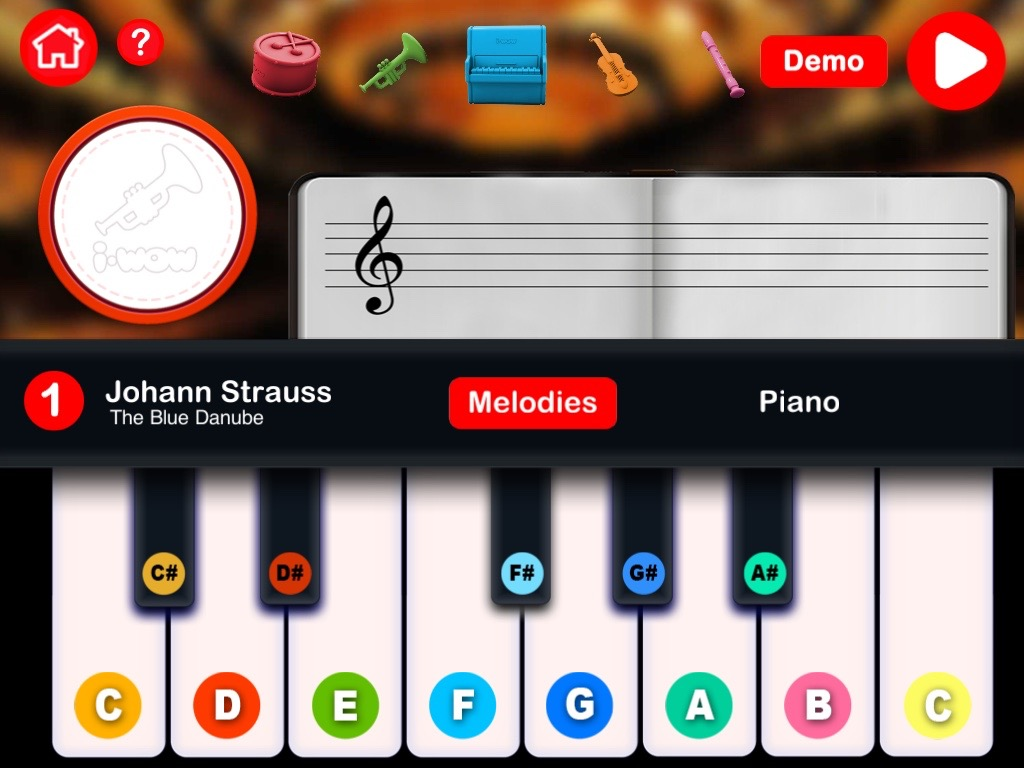
\includegraphics[width=350pt]{graphics/use-case/playing_piano_screen.jpg}
  \vspace{0.05cm}
  \caption{Playing piano screen}
  \label{fig:playing_piano_screen}
  \vspace{0.6cm}

  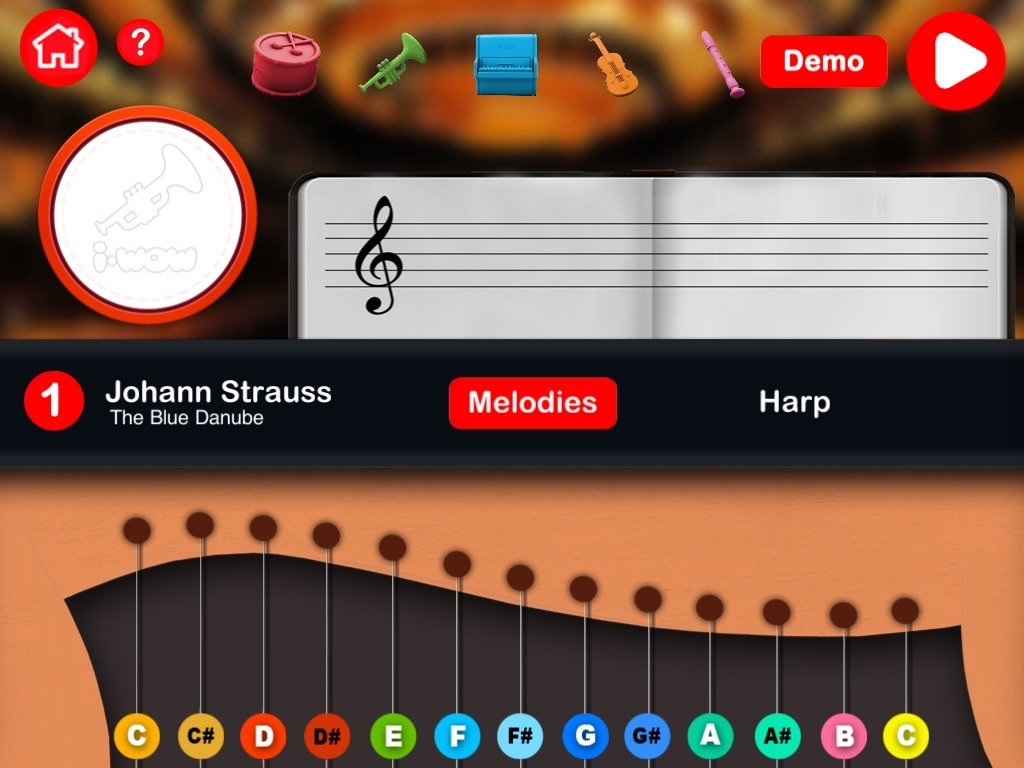
\includegraphics[width=350pt]{graphics/use-case/playing_harp_screen.jpg}
  \vspace{0.05cm}
  \caption{Playing harp screen}
  \label{fig:playing_harp_screen}
\end{figure}

\section{Conducting game mode}

\begin{figure}[ht!]
  \centering
  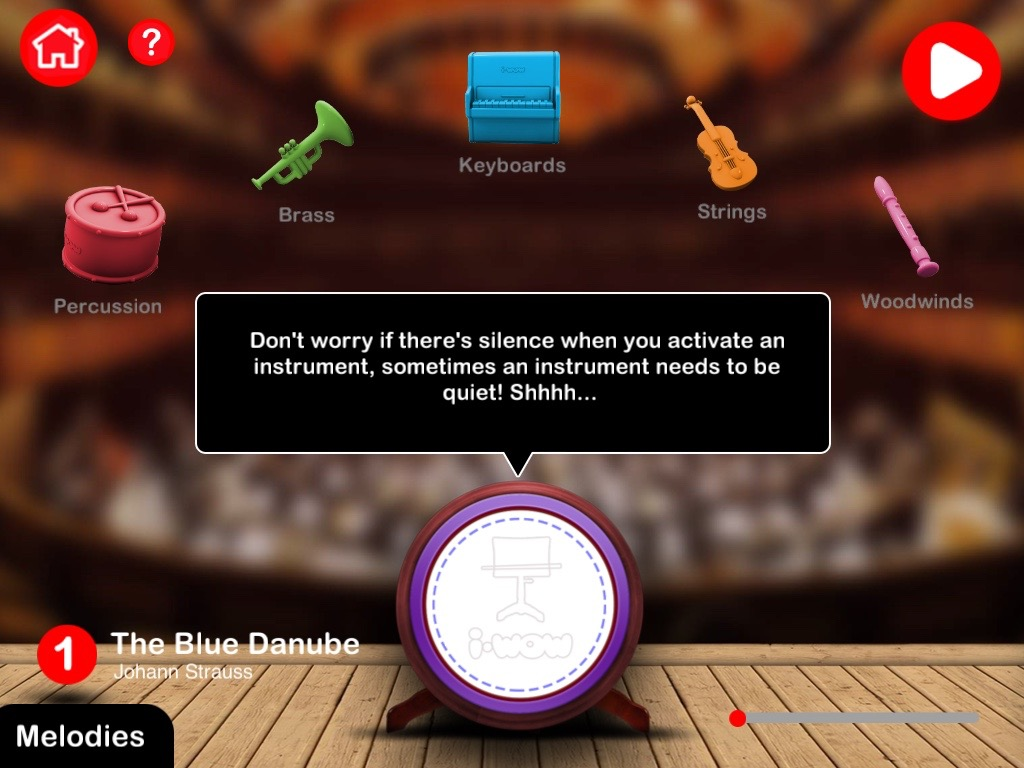
\includegraphics[width=350pt]{graphics/use-case/conducting_home_screen.jpg}
  \vspace{0.05cm}
  \caption{Conducting game mode access screen}
  \label{fig:conducting_home_screen}
  \vspace{0.6cm}

  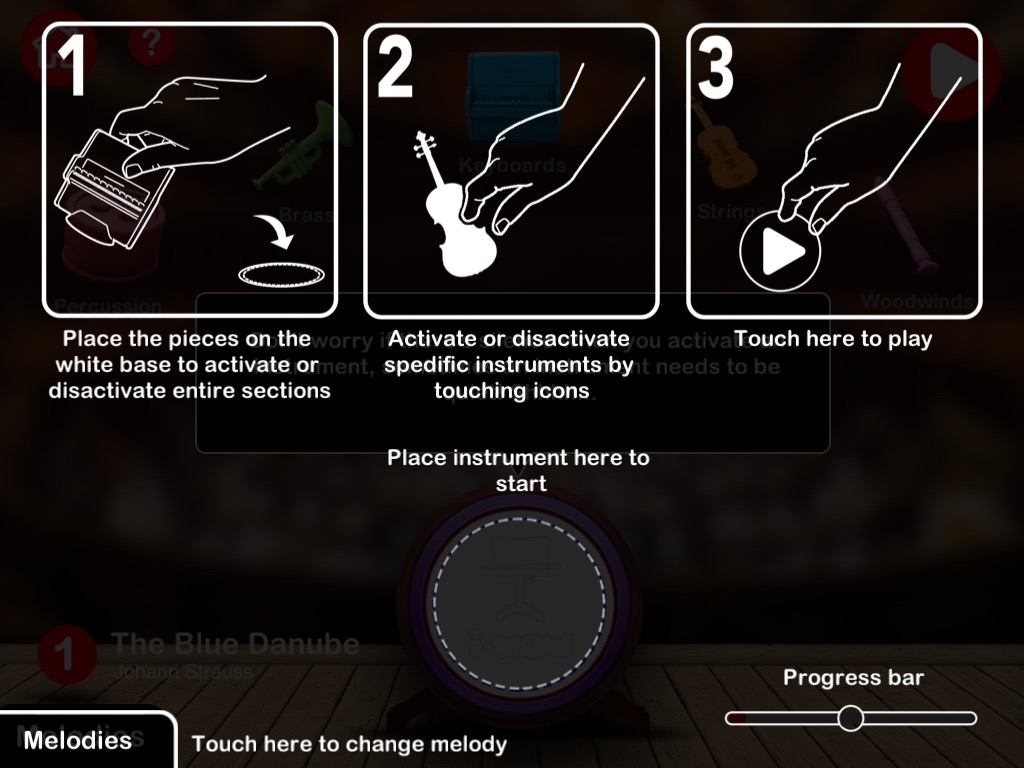
\includegraphics[width=350pt]{graphics/use-case/help_conducting_screen.jpg}
  \vspace{0.05cm}
  \caption{Help information conducting orchestra game mode}
  \label{fig:help_conducting_screen}
\end{figure}

\begin{figure}[ht!]
  \centering
  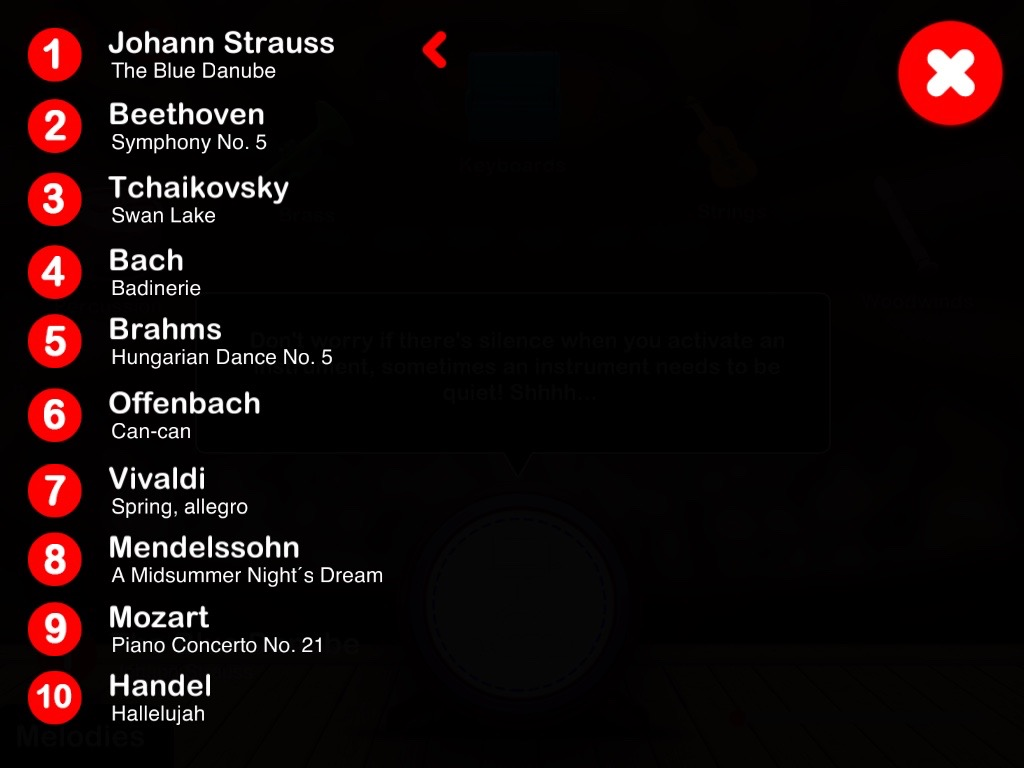
\includegraphics[width=350pt]{graphics/use-case/conducting_melodies_screen.jpg}
  \vspace{0.05cm}
  \caption{Melodies selection in the conducting orchestra game mode}
  \label{fig:conducting_melodies_screen}
  \vspace{0.6cm}

  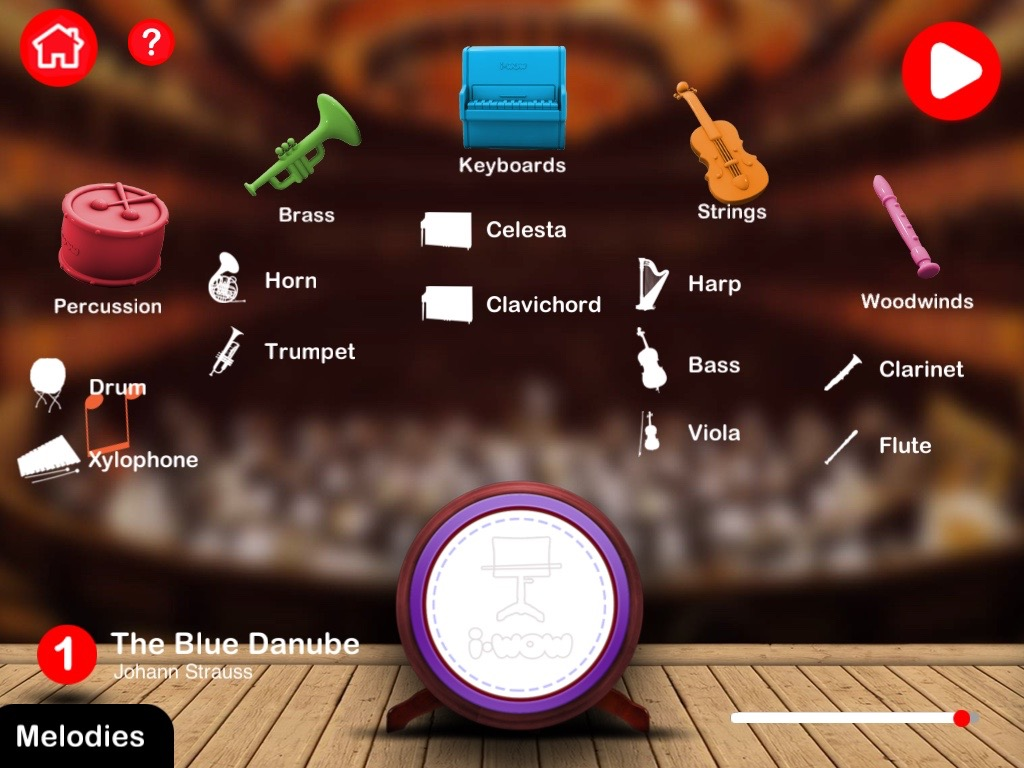
\includegraphics[width=350pt]{graphics/use-case/conducting_all_stop_screen.jpg}
  \vspace{0.05cm}
 \caption{Conducting orchestra screen with all instruments activated}
  \label{fig:conducting_all_stop_screen}
\end{figure}

\section{Discovering game mode}


\phantomsection
\addcontentsline{toc}{chapter}{Bibliography}
\bibliographystyle{ieeetr}
{
\small
\bibliography{biblio/ref}
}
\cleardoublepage
\end{document}